        %%******************************************%%
        %%                                          %%
        %%        Modello di tesi di laurea         %%
        %%            di Andrea Giraldin            %%
        %%                                          %%
        %%             2 novembre 2012              %%
        %%                                          %%
        %%******************************************%%

\begin{document}
    \frontmatter
    \begin{titlepage}
    \begin{center}
        \begin{LARGE}
            \textbf{\myUni}\\
        \end{LARGE}

        \vspace{10pt}

        \begin{Large}
            \textsc{\myDepartment}\\
        \end{Large}

        \vspace{10pt}

        \begin{large}
            \textsc{\myFaculty}\\
        \end{large}

        \vspace{30pt}
        \begin{figure}[htbp]
            \centering
            
\includegraphics[height=6cm]{unipd-logo}
        \end{figure}
        \vspace{30pt}

        \begin{LARGE}
            \textbf{\myTitle}\\
        \end{LARGE}

        \vspace{10pt}

        \begin{large}
            \textsl{\myDegree}\\
        \end{large}

        \vspace{40pt}

        \begin{large}
            \begin{flushleft}
                \textit{Relatore}\\
                \vspace{5pt}
                \profTitle\ \myProf
            \end{flushleft}

            % You can tweak the spacing to have professor and student names on the same line
            % useful if the page is broken by a long thesis title and you need more space
            % \vspace{-52pt}

            \begin{flushright}
                \textit{Laureando}\\
                \vspace{5pt}
                \myName \\
                \vspace{5pt}
                \textit{Matricola} \myID
            \end{flushright}
        \end{large}

        \vspace{40pt}

        \line(1, 0){338} \\
        \begin{normalsize}
            \textsc{Anno Accademico \myAA}
        \end{normalsize}
    \end{center}
\end{titlepage}

    \clearpage
\phantomsection
\thispagestyle{empty}

\hfill
\vfill

\noindent\myName: \textit{\myTitle,}
\myDegree,
\textcopyright\ \myTime.

    %\cleardoublepage
\phantomsection
\thispagestyle{empty}
\pdfbookmark{Dedica}{Dedica}

\vspace*{3cm}

\begin{center}
    Lorem ipsum dolor sit amet, consectetuer adipiscing elit. \\ \medskip
    --- Oscar Wilde
\end{center}

\medskip

\begin{center}
    Dedicato a ...
\end{center}

    \cleardoublepage
\phantomsection
\pdfbookmark{Sommario}{Sommario}
\begingroup
\let\clearpage\relax
\let\cleardoublepage\relax
\let\cleardoublepage\relax

\chapter*{Sommario}

Il presente documento descrive il lavoro svolto durante il periodo di stage, della durata di circa trecento ore, dal laureando Pinco Pallino presso l'azienda Azienda S.p.A.
Gli obbiettivi da raggiungere erano molteplici.\\
In primo luogo era richiesto lo sviluppo di ...
In secondo luogo era richiesta l'implementazione di un ...
Tale framework permette di registrare gli eventi di un controllore programmabile, quali segnali applicati
Terzo ed ultimo obbiettivo era l'integrazione ...

%\vfill

%\selectlanguage{english}
%\pdfbookmark{Abstract}{Abstract}
%\chapter*{Abstract}

%\selectlanguage{italian}

\endgroup

\vfill

    %\cleardoublepage
\phantomsection
\pdfbookmark{Ringraziamenti}{ringraziamenti}

\begin{flushright}{
    \slshape
    ``Life is really simple, but we insist on making it complicated''} \\
    \medskip
    --- Confucius
\end{flushright}


\bigskip

\begingroup
\let\clearpage\relax
\let\cleardoublepage\relax
\let\cleardoublepage\relax

\chapter*{Ringraziamenti}

\noindent \textit{Innanzitutto, vorrei esprimere la mia gratitudine al Prof. \myProf, relatore della mia tesi, per l'aiuto e il sostegno fornitomi durante la stesura del lavoro.}\\

\noindent \textit{Desidero ringraziare con affetto i miei genitori per il sostegno, il grande aiuto e per essermi stati vicini in ogni momento durante gli anni di studio.}\\

\noindent \textit{Ho desiderio di ringraziare poi i miei amici per tutti i bellissimi anni passati insieme e le mille avventure vissute.}\\
\bigskip

\noindent\textit{\myLocation, \myTime}
\hfill \myName

\endgroup

    \cleardoublepage
\pdfbookmark{\contentsname}{tableofcontents}
\setcounter{tocdepth}{2}
\tableofcontents
%\markboth{\contentsname}{\contentsname}
\clearpage

\begingroup
    \let\clearpage\relax
    \let\cleardoublepage\relax
    \let\cleardoublepage\relax

    % Figures list
    \phantomsection
    \pdfbookmark{\listfigurename}{lof}
    \listoffigures

    \vspace*{8ex}

    % Tables list
    \phantomsection
    \pdfbookmark{\listtablename}{lot}
    \listoftables

    \vspace*{8ex}
\endgroup

\cleardoublepage

    \cleardoublepage

    \mainmatter
    \chapter{Contesto aziendale}
\label{cap:contestoAziendale}

\section{Wintech S.p.A.}
Winning Technologies, in sigla Wintech S.p.A., venne fondata nel 1987 dall'attuale amministratore delegato Massimo Gallotta.\\
Essa si occupa di \gls{system integration} nell'ambito delle tecnologie dell'informazione e della comunicazione, ovvero unisce ed integra diverse tecnologie e sistemi informatici al fine di ottenere un prodotto coordinato e maggiormente gestibile.\\
L'azienda, la quale conta più di 90 dipendenti, ha sede principale situata a Padova ma, grazie al suo sviluppo, ha acquisito filiali a Milano e a Bassano del Grappa.\\
Wintech ha stretto svariate \emph{partnership} con aziende \emph{leader} di mercato come IBM, Microsoft e HP grazie anche alla propria affidabilità e solidità finanziaria.\\ 
Inoltre, possiede diverse società partecipate, tra cui Sistemi S.p.A., con le quali è attiva una forte collaborazione.\\
I clienti di Wintech comprendono grandi imprese (tra cui BMW, Helvetia e Lindt), PMI, professionisti, aziende assicurative e imprese finanziarie. 

\section{Prodotti e servizi}
\subsection{Servizi}
I servizi offerti da Wintech comprendono diverse aree tecnologiche:
\begin{itemize}
	\item \textbf{Infrastrutture \gls{IT}}: vengono offerte soluzioni per modernizzare e gestire le infrastrutture aziendali sfruttando tecnologie \gls{cloud}, progettazioni di reti \gls{LAN}/\gls{WAN}, gestione di \emph{backup} sicuri e supporto \gls{IT} conforme agli standard \gls{ITIL}. 
	\item \textbf{Automazione di processi di \emph{Business}}: vengono forniti strumenti per automatizzare i processi aziendali come flussi approvativi, gestione documentale e progetti \gls{DevOps}.
	\item \textbf{\emph{Cyber} sicurezza}: viene fornita protezione contro i rischi informatici mediante difesa delle reti e dei dispositivi, segmentazione della rete, servizi gestiti e soluzioni di \gls{disaster recovery} per garantire la continuità aziendale. 
	\item \textbf{Soluzioni \gls{ERP}}: vengono sviluppati sistemi per la gestione delle risorse aziendali come automazioni per le Risorse Umane, sistema di gestione dei clienti (\emph{Customer Relationship Management}), soluzioni gestionali per la produzione industriale, soluzioni per industria 4.0/5.0.\\
\end{itemize}
Viene offerta consulenza al cliente al fine di fornire supporto tecnico e comprendere le sue necessità.\\
Successivamente viene identificata una soluzione adeguata, la quale può essere sviluppata partendo da un prodotto aziendale già consolidato apportando le opportune personalizzazioni, oppure realizzando un prodotto nuovo.\\
In seguito allo sviluppo di un prodotto, vengono forniti servizi di formazione, assistenza e manutenzione dello stesso. 

\subsection{Prodotti}
I principali prodotti offerti dall'azienda sono: 

\subsubsection*{Spring}
Supporta le \gls{PMI} gestendo le informazioni relative alle attività di diverse aree aziendali come: 

\begin{itemize}
    \item Amministrativa 
    \item Vendite 
    \item Acquisti 
    \item Logistica e magazzino
    \item Analisi e \emph{reporting}
    \item Gestione documentale
\end{itemize}

\subsubsection*{Profis}
Fornisce servizi legati alle aree di attività dello studio del commercialista come: 
\begin{itemize}
    \item Area fiscale dei bilanci 
    \item Contabilità e digitalizzazione dei processi di fatturazione  
\end{itemize}

\subsubsection*{Studio}
Offre servizi legati all'organizzazione e alla gestione dello studio professionale come:
\begin{itemize}
    \item Calendari condivisi  
    \item Gestione efficiente delle pratiche 
    \item Emissione di parcelle  
    \item Fatture elettroniche 
\end{itemize}

\subsubsection*{Job}
Fornisce servizi legati alla gestione del personale come: 
\begin{itemize}
    \item Gestione delle presenze  
    \item Amministrazione delle Risorse Umane  
    \item Elaborazioni dei cedolini 
    \item Analisi sui costi del personale
\end{itemize}

\subsubsection*{Sportello}
Propone servizi legati alla gestione dei clienti come:  
\begin{itemize}
    \item Gestione della fatturazione online 
    \item Gestione degli incassi e dei pagamenti 
    \item Condivisione, validazione e conservazione digitale dei documenti  
\end{itemize}

\subsubsection*{eSolver}
Mette a disposizione servizi legati alla gestione dei processi per aziende di produzione, di servizi, di commercio all'ingrosso e al dettaglio. 
Le principali funzionalità comprendono: 
\begin{itemize}
    \item Amministrazione e finanza 
    \item Acquisti e rapporti di fornitura 
    \item Vendite e attività commerciale 
    \item Logistica
    \item Archiviazione e conservazione documentale
    \item Gestione risorse produttive 
    \item Produzione manifatturiera  
    \item Controllo di gestione 
    \item \emph{Reporting} e analisi 
\end{itemize}

\subsubsection*{WOW}
\label{WOW}
“\emph{World Of Wintech}” (WOW) viene considerato non solo un utile prodotto per i clienti, ma soprattutto un potente strumento gestionale aziendale utilizzato da tutti i dipendenti.\\ 
Essa è una soluzione basata interamente sul \gls{cloud}, altamente personalizzabile ed integrabile con i sistemi gestionali e applicativi già in possesso da un cliente.\\
WOW permette di utilizzare svariati moduli gestionali in un'unica interfaccia utente e di gestire i documenti grazie alla piattaforma di \gls{back-end} FileNet - IBM, permettendo operazioni di collaborazione in tempo reale.\\\\
I principali moduli che lo compongono sono: 

\begin{itemize}
    \item \textbf{Home}: organizzazione delle risorse aziendali interne. 
    \item \textbf{Opportunità}: tracciamento delle trattative commerciali. 
    \item \textbf{Marketing}: gestione delle azioni di \emph{marketing}. 
    \item \textbf{Campagne commerciali}: assegnazione delle attività e gestione campagne commerciali.
    \item \textbf{Anagrafiche}: profilazione clienti e contatti aziendali. 
    \item \textbf{Commesse}: gestione informazioni anagrafiche di commessa al fine di categorizzare i documenti archiviati.
    \item \textbf{Add-In O365}: connessione con Outlook365 per l'archiviazione dei messaggi di posta elettronica.
    \item \textbf{Registro accessi}: gestione degli accessi in azienda da parte di ospiti e collaboratori.
    \item \textbf{Documenti}: archiviazione dei documenti mediante la piattaforma IBM e l'integrazione con Microsoft365.\\
\end{itemize}
\hyperref[WOW]{WOW} si integra con il prodotto eSolver al fine di gestire tutte le principali aree di interesse aziendale. 

\section{Processi aziendali}
\subsection{Agile}
Grazie all'utilizzo di \hyperref[WOW]{WOW} e alle politiche aziendali, è molto forte la collaborazione e la condivisione di informazioni tra i dipendenti. Il tutto è reso maggiormente dinamico ed efficiente grazie all'adozione della metodologia \emph{Agile}.\\
Essa è un approccio alla gestione progettuale che promuove la collaborazione e il dialogo tra membri del \emph{team} e con i clienti al fine di condividere costantemente \emph{feedback} e rispondere prontamente ai cambiamenti.\\\\
I quattro valori che descrivono la filosofia \emph{Agile} sono:
\begin{itemize}
    \item Gli individui e le interazioni più che i processi e gli strumenti 
    \item Il \emph{software} funzionante più che la documentazione esaustiva  
    \item La collaborazione col cliente più che la negoziazione del contratto 
    \item Rispondere al cambiamento più che seguire un piano\\
\end{itemize}
In Wintech viene adottato il \emph{framework} \emph{Agile} “\emph{Scrum}” per la gestione dei progetti.\\
Esso prevede una divisione temporale dell'avanzamento dei lavori organizzata per “\emph{Sprint}”, i quali in azienda hanno una durata variabile di circa un mese ciascuno.\\
All'inizio di ogni \emph{Sprint} esso viene pianificato definendo tutte le attività da svolgere.\\ 
Quotidianamente è previsto un breve incontro tra i membri del \emph{team} in modo da confrontarsi sullo stato di avanzamento dei lavori e su eventuali problemi riscontrati.\\
Al termine dello \emph{Sprint} viene fatta una revisione per analizzare i risultati ottenuti e avviene un'analisi retrospettiva al fine di far emergere gli aspetti positivi e quelli migliorabili riguardo il suo svolgimento, la collaborazione del \emph{team} e l'utilizzo degli strumenti forniti.\\\\
Il \emph{framework} adottato prevede tre figure fondamentali: 
\subsubsection*{Product Owner}
Colui che si focalizza sulle esigenze aziendali, dei clienti e di mercato. Egli definisce le attività da compiere e la loro priorità.
In azienda tale ruolo è responsabilità del \gls{project manager}. 

\subsubsection*{Scrum Master}
Colui che organizza le risorse per la pianificazione dello \emph{Sprint} e coordina lo svolgimento delle procedure e cerimonie \emph{Scrum} garantendo una corretta applicazione delle sue filosofie.
In azienda tale ruolo è responsabilità del \gls{project manager}. 

\subsubsection*{Team di sviluppo}
Il gruppo di lavoro, il quale gode di una buona autonomia nell'avanzamento e assegnazione dei lavori, è composto da una decina di membri con diverse competenze. Tra loro è presente una forte collaborazione e dialogo in modo da condividere le proprie conoscenze e progredire con lo stato dei lavori in modo efficace. 

\begin{figure}[htbp] 
    \centering 
    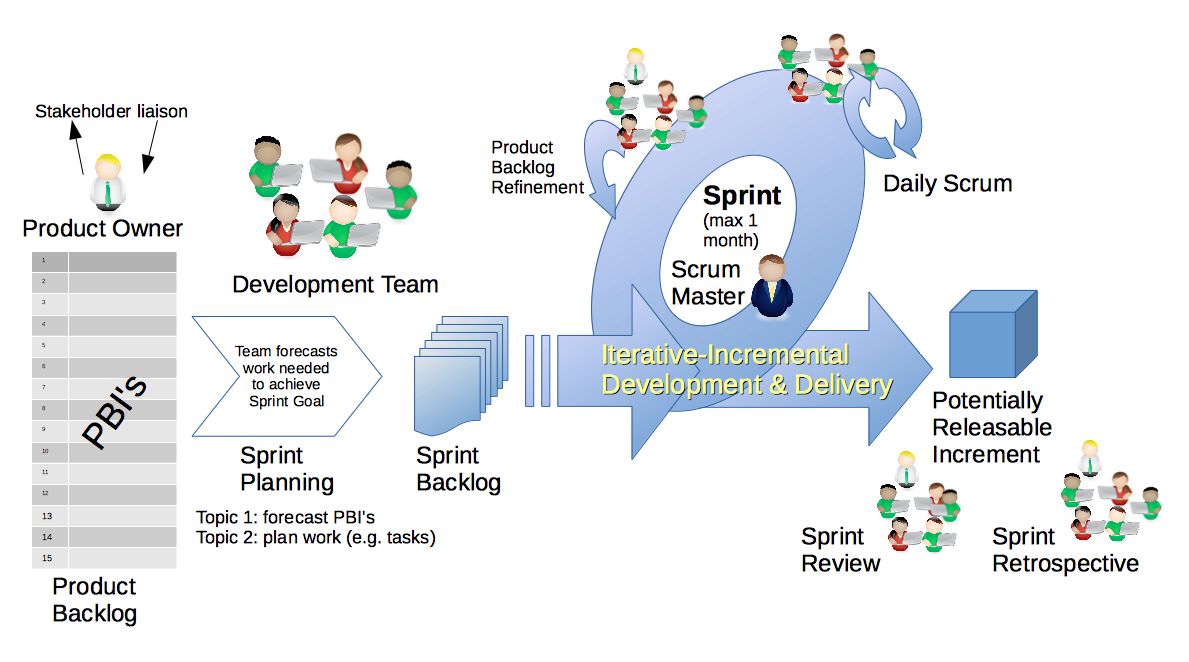
\includegraphics[width=1\columnwidth]{scrum_Framework} 
    \caption{Organizzazione framework Scrum.}
    \label{fig:scrum_framework}
    \vspace{1mm}
    Fonte: \url{https://commons.wikimedia.org/wiki/File:Scrum_Framework.png}.
\end{figure}



\subsection{\glslink{unità operativa}{Unità operative}}
Le principali \glslink{unità operativa}{unità operative} in cui è strutturata Wintech sono:

\subsubsection*{Applicazioni}
Formata da un gruppo di consulenti applicativi i quali si occupano di consulenza, integrazione e assistenza sui \emph{software} gestionali aziendali nei confronti dei clienti. 

\subsubsection*{Soluzioni}
Comprende programmatori con competenze trasversali in grado di definire, progettare e realizzare le soluzioni necessarie per soddisfare le richieste dei clienti. 

\subsubsection*{Tecnologie}
Al suo interno persone con competenza sistemistica monitorano e gestiscono i \emph{server} aziendali al fine di garantire continuità operativa a tutti i clienti in \gls{cloud}. Il personale si dedica all'assistenza dei clienti sia da remoto che in sede, proponendo componenti \emph{hardware} adatte alle esigenze. 

\subsubsection*{Ricerca e Sviluppo}
Composta da un \emph{team} di programmatori avente una maggiore libertà in termini di sperimentazione tecnologica e metodologica. Durante il corso dello \emph{stage} ho fatto parte di questa \gls{unità operativa}. 

\subsection{Documenti e Certificazioni}
Durante il ciclo di vita di un progetto vengono generati un insieme di documenti atti a descriverlo e a normare le attività in esso svolte.\\
I documenti che descrivono le procedure e i metodi da adottare per garantire sicurezza e qualità al prodotto sono spesso comuni a più progetti, pertanto, essi vengono duplicati e modificati solo nei casi in cui le tecnologie o le circostanze rendono tali modifiche necessarie.\\
Tra questi documenti ci sono i “Documenti di sviluppo sicuro” i quali normano le procedure legate al ciclo di vita del progetto e alle buone pratiche da adottare.\\ 
Differentemente, alcuni documenti devono venire prodotti più specificatamente per ogni progetto. Tra questi sono presenti: l'analisi dei requisiti, lo schema architetturale, le criticità, il manuale utente e di installazione, il verbale di collaudo e il “\emph{Bill of Material}” contenente tutti i \emph{software} di terze parti necessari all'utilizzo.\\\\
I processi aziendali definiti hanno reso possibile l'ottenimento delle certificazioni UNI CEI ISO/IEC 27001:2017 IAF 33 e UNI EN ISO 9001:2015 IAF 33,39,37 le quali attestano rispettivamente la conformità del sistema di gestione per la sicurezza delle informazioni e la qualità della gestione aziendale in termini di efficacia, efficienza e soddisfazione dei clienti. 


\section{Tecnologie utilizzate}
All'interno dell'azienda, più specificatamente nelle \glslink{unità operativa}{unità operative} Ricerca e Sviluppo e Soluzioni, vengono utilizzate le seguenti tecnologie: 
\begin{itemize}
    \item Per la pianificazione e il monitoraggio delle attività progettuali vengono utilizzate piattaforme dedicate come Microsoft Planner e Taiga, strumenti versatili che permettono di organizzare \glslink{caso d'uso}{casi d'uso} e \emph{task} in modo collaborativo ed efficiente. 
    \item La collaborazione tra i membri del personale è agevolata da strumenti come Microsoft Teams e Outlook, i quali permettono di: scambiare ed organizzare messaggi ed \emph{e-mail}, gestire eventi come riunioni e \emph{meeting} in un apposito calendario sincronizzato ed effettuare videochiamate per agevolare l'interazione e la collaborazione tra colleghi. 
    \item Gli sviluppatori possono scegliere liberamente gli ambienti di sviluppo più adatti alle loro esigenze, anche se i principali strumenti utilizzati sono Visual Studio Code e IntelliJ IDEA, che offrono supporto per molteplici linguaggi di programmazione e \emph{framework}. 
    \item I sistemi operativi prevalentemente utilizzati in azienda sono Windows 11 e Windows 10 in modo da garantire un ambiente compatibile con la maggior parte degli strumenti \emph{software}. 
    \item Il versionamento del codice sorgente è gestito tramite Git, con il supporto di piattaforme come GitHub e GitLab, che assicurano un controllo efficace delle versioni e agevolano la collaborazione. 
    \item Per il controllo e l'automazione del ciclo di vita del \emph{software} viene utilizzato Jenkins, uno strumento che permette di ottimizzare i processi di sviluppo e distribuzione tramite \gls{Continuous Integration} e \gls{Continuous Deployment}. 
    \item La qualità del \emph{software} è garantita attraverso strumenti come SonarQube per l'analisi statica del codice, JUnit per i \emph{test} di unità ed integrazione, JMeter per i \emph{test} di carico e \emph{stress test}.\\
    Per migliorare il processo di \emph{test} viene utilizzato, dove necessario, il \emph{framework} Mockito per simulare il comportamento di specifici componenti o dipendenze esterne.\\
    Viene inoltre utilizzato lo strumento OWASP ZAP per testare il soddisfacimento di molteplici requisiti di sicurezza. 
    \item Le tecnologie principali utilizzate per la creazione e gestione della documentazione aziendale comprendono l'insieme Microsoft Office 365 mentre, per lo sviluppo \emph{software}, vengono utilizzati soprattutto il linguaggio Java e il \emph{framework} Angular. 
    \item Per la gestione e configurazione di un \emph{server web} e di basi di dati, vengono utilizzate rispettivamente Apache Web server e SQL server. 
\end{itemize}

\section{Innovazione aziendale}
L'azienda non sottovaluta l'importanza dell'innovazione in un ambiente lavorativo in costante aggiornamento come quello \gls{IT}. Lo dimostra l'importanza che viene data all'\gls{unità operativa} Ricerca e Sviluppo, alla quale ho partecipato approfondendo tecnologie nuove per l'azienda e valutando nuovi approcci organizzativi. Questi ultimi includono l'implementazione, per le nuove tecnologie adottate, di metodologie \gls{DevOps}. Tali processi atti all'automazione vengono già applicati per tecnologie consolidate aumentando l'efficacia, l'efficienza e la qualità dei lavori.\\
Wintech riconosce il valore aggiunto che i giovani possono portare e, da diversi anni, offre la possibilità di svolgere \emph{stage} universitari per formare e inserire nel mondo del lavoro studenti prossimi alla laurea.\\
Spesso, per questi ultimi, si concretizza l'opportunità di proseguire lavorativamente i rapporti con l'azienda, pertanto, il \emph{team} di sviluppo è caratterizzato da un'età media relativamente giovane, pur mantenendo al suo interno figure con consolidata esperienza.\\ 
Inoltre, al fine di accrescere le potenzialità delle proprie risorse, l'azienda fornisce corsi di formazione mirati per il personale.

    \chapter{Progetto di \emph{stage}}
\label{cap:progettoDiStage}

\section{Visione aziendale}
\subsection{Rapporto dell'azienda con gli \emph{stage}}
Wintech identifica gli \emph{stage} universitari come strumenti utili alla formazione professionale dei laureandi al fine di renderli risorse produttive non solo per il periodo di \emph{stage} definito, ma soprattutto per il periodo successivo. È infatti consuetudine per l'azienda decidere di proseguire i rapporti lavorativi con gli studenti, pertanto, è nel suo interesse rendersi disponibile fornendo approfondimenti e attività formative in ambito tecnologico e riguardo i processi aziendali.\\\\
Per proporre la propria disponibilità e avere un primo contatto con gli studenti, Wintech partecipa da diversi anni all'evento dedicato STAGEIT promosso da Confindustria Veneto Est in collaborazione con i Dipartimenti di Scienze Statistiche, Matematica e Ingegneria dell'Informazione dell'Università di Padova, al fine di favorire l'incontro tra aziende associate e gli studenti per esporre i progetti \gls{ICT} proposti.\\\\
Successivamente, organizza colloqui conoscitivi al fine di spiegare la propria visione aziendale e i propri progetti di \emph{stage} agli studenti.\\
Tali progetti non sono pensati per essere esclusivamente didattici ma forniscono un tangibile valore all'azienda in quanto si basano sulle tecnologie e metodologie da loro realmente utilizzate o che prevedono di integrare.\\
Lo stagista non è pertanto visto solo come uno studente ma viene integrato al \emph{team} di sviluppo con il quale lavora a stretto contatto acquisendo nuove competenze sia collaborativamente che autonomamente.\\

\subsection{Progetti proposti}
I progetti di \emph{stage} proposti dall'azienda, contestualmente al periodo della nostra collaborazione, derivano dal valore aggiunto che l'automazione dei processi aziendali può portare in ambiti di pianificazione progettuale, per ambienti di sviluppo consolidati e per tecnologie oggetto di ricerca.\\
Tale processo permette di realizzare efficientemente prodotti con maggiore qualità riducendo sensibilmente i tempi e i costi dei lavori.\\
Inoltre, automatizzare attività ben definite riduce sensibilmente la possibilità di introduzione manuale di errori e ne permette una rapida individuazione.\\
Durante la durata dello \emph{stage}, gli stagisti hanno collaborato tra loro più volte trovando dei punti di incontro tra i propri progetti e rimanendo aggiornati riguardo ai rispettivi risultati ottenuti tramite appositi incontri.\\\\
I progetti proposti in questione sono: 

\subsubsection*{Applicativi di DevOps in ambito Sistemi e Office365}
\label{mioStage}
Lo scopo dello \emph{stage} da me svolto è compiere un'analisi per verificare l'applicabilità delle pratiche di \gls{DevOps} su progetti basati sull'utilizzo di tecnologie Office365, più specificatamente ai programmi Power Automate e Power Apps, con lo scopo di integrarle nell'infrastruttura aziendale.\\
Le soluzioni individuate durante la ricerca vengono introdotte nel contesto aziendale tramite fasi di sviluppo sia implementando tali risultati allo sviluppo di reali applicazioni aziendali realizzate collaborando con il \emph{team}, sia realizzando \emph{Proof of Concept} (PoC), ovvero elementi dimostrativi realizzati al fine di provare la fattibilità di un prodotto mediante l'utilizzo delle tecnologie e degli strumenti definiti. Esso rappresenta quindi una versione di prova prototipale e non ha lo scopo di divenire il prodotto finale ma viene realizzato a supporto dell'analisi progettuale.
\begin{figure}[htbp] 
    \centering 
    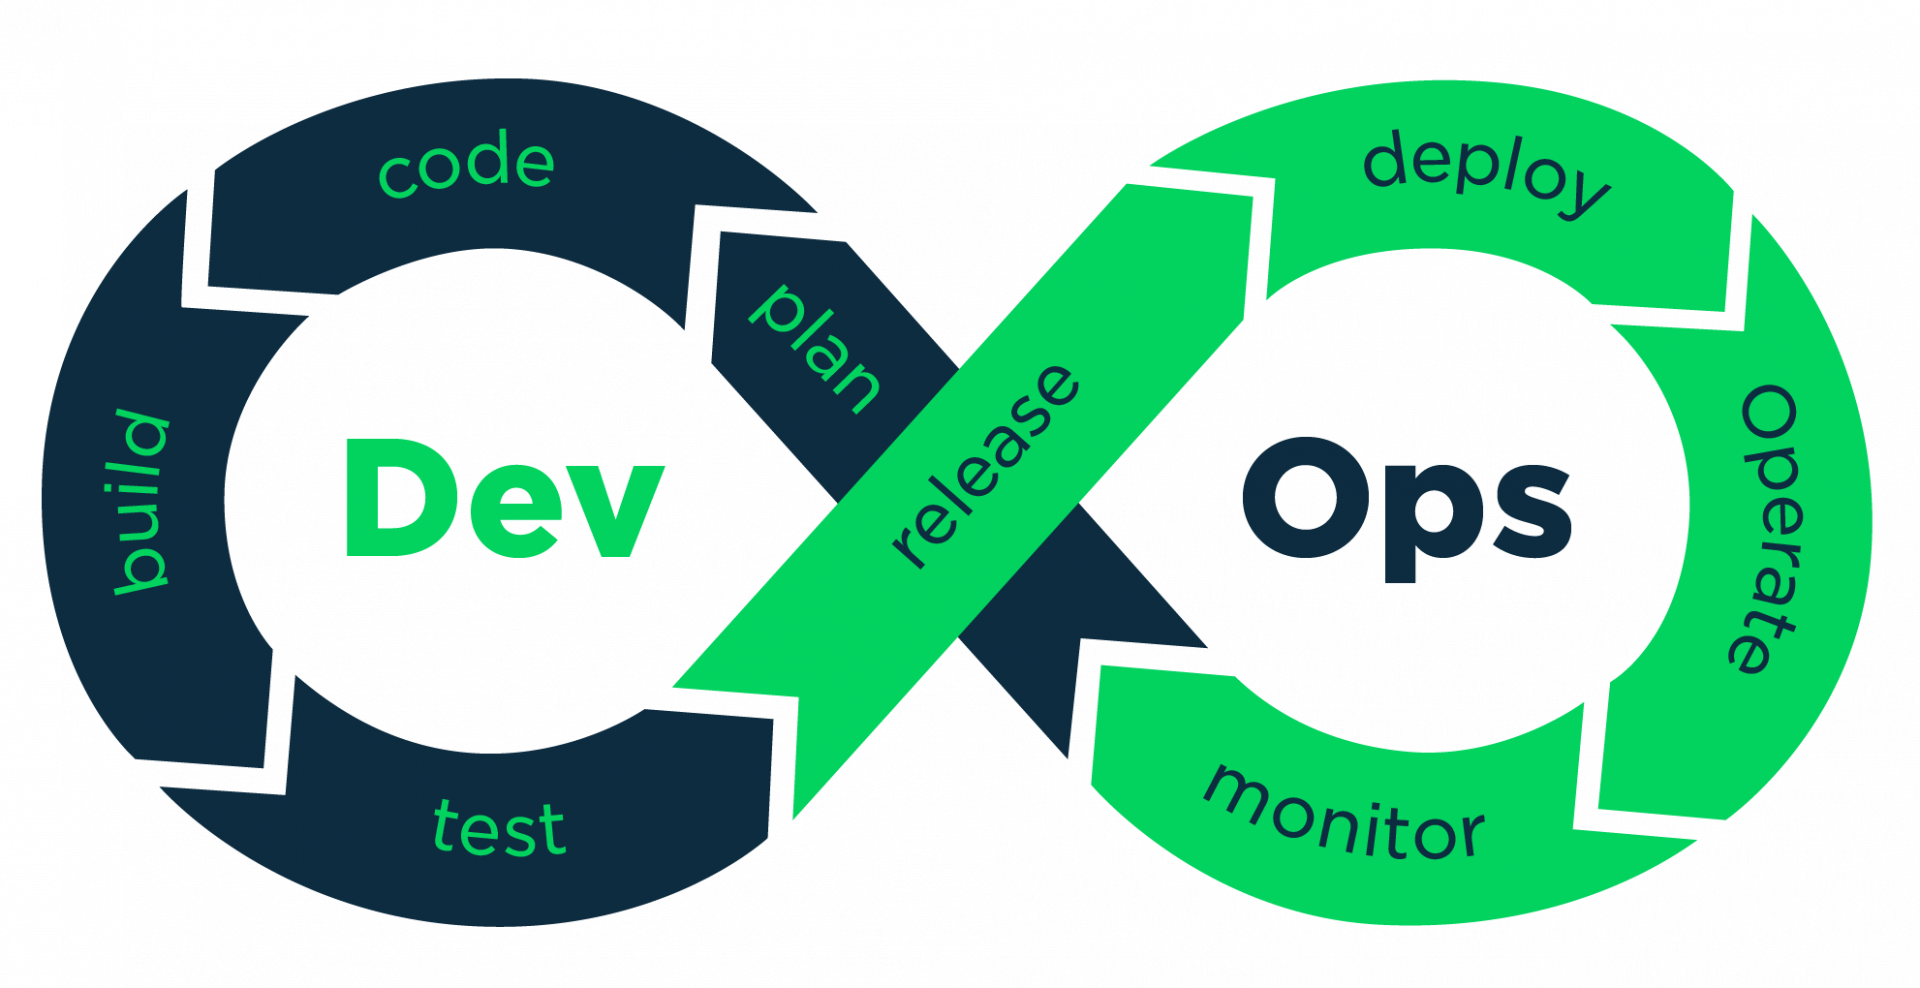
\includegraphics[width=0.8\columnwidth]{DevOps}
    \caption{Ciclo e fasi di DevOps.} 
    \label{fig:DevOps}
\end{figure}

\subsubsection*{Integrazione sistemi di pianificazione di progetto}
Lo scopo dello \emph{stage} è compiere un'analisi per verificare l'utilizzo degli strumenti di pianificazione aziendale, nello specifico Planner e Taiga, e lo sviluppo di una soluzione atta ad automatizzare la comunicazione e sincronizzazione di tali strumenti.\\
Per raggiungere tale obiettivo è presente la possibilità di utilizzare le \emph{Application Programming Interface} (API): In italiano "Interfacce di Programmazione dell'Applicazione", rappresentano un insieme di procedure che permettono la comunicazione e lo scambio di dati tra diversi componenti \emph{software}. L'utilizzo di API permette di semplificare l'integrazione tra prodotti e servizi informatici rendendo disponibili funzionalità esterne senza doverne conoscere l'effettiva implementazione.

\subsubsection*{Applicativi di DevOps in ambito Sistemi}
\label{stageDavide}
Lo scopo dello \emph{stage} è compiere un'analisi per verificare l'applicabilità delle pratiche di \gls{DevOps} all'ambiente di sviluppo \gls{Sistemi}, con lo scopo di integrarle nell'infrastruttura aziendale in ambiti ben definiti.\\
Le soluzioni individuate durante la ricerca vengono introdotte nel contesto aziendale tramite fasi di sviluppo. 


\section{\emph{Stage} da me svolto}
\hyperref[mioStage]{Applicativi di DevOps in ambito Sistemi e Office365}
\subsection{Obiettivi progettuali}
Gli obiettivi dello \emph{stage}, come dichiarati nel documento “Progetto Formativo” generato all'inizio del suo svolgimento, sono divisi in categorie:
\begin{enumerate}
	\item[O -]requisiti obbligatori, vincolanti in quanto obiettivo primario richiesto dall'azienda.
    \item[D -]requisiti desiderabili, non strettamente necessari ma dal riconoscibile valore aggiunto.
    \item[F -]requisiti facoltativi / opzionali, rappresentanti un valore aggiunto non strettamente competitivo.\\\\
\end{enumerate}
Essi sono:

\begin{table}[htbp]
    \label{tab:obiettiviProgettuali}
    \renewcommand{\arraystretch}{1.5}
    \begin{tabularx}{\textwidth}{|l|X|l|}
    \hline
    \textbf{Codice} & \textbf{Descrizione}\\
    \hline
    O1    & Mappatura delle funzionalità possibili tramite l'adozione dei due applicativi \gls{Sistemi} e Office365.\\
    \hline O1.1  & Analisi approfondita del sistema e delle parti interessate.\\
    \hline O1.2  & Studio delle modalità di lavoro degli utenti.\\
    \hline O1.3  & Produzione di una completa documentazione di uso.\\
    \hline O2  & Personalizzazione e integrazione: individuare le modalità di utilizzo.\\
    \hline
    \hline D1  & Analisi dei requisiti per l'integrazione aziendale della metodologia \gls{DevOps} in ambito \GLS{Sistemi} e Office365.\\
    \hline D2  & Produzione di una completa documentazione progettuale.\\
    \hline
    \hline F1  & Realizzazione di \emph{Proof of concept}.\\
    \hline F2  & Presentazione interna.\\
    \hline F3  & Predisposizione della documentazione.\\
    \hline
    \end{tabularx}
    \caption{Tabella degli obiettivi progettuali.}
\end{table}%
\newpage \noindent Tali obiettivi si traducono nelle seguenti aspettative a fine progetto: 
\subsubsection*{Obbligatori}
\begin{itemize}
    \item Documentazione che determini se le metodologie \gls{DevOps} aziendali siano applicabili in ambito \gls{Sistemi} eOffice365
    \item Configurazioni e \emph{software} realizzati per determinare l'applicazione del \gls{DevOps} aziendale in ambito \gls{Sistemi} e Office365
\end{itemize}
\subsubsection*{Desiderabili}
\begin{itemize}
    \item Documentazione di sviluppo sicuro annotata con l'esperienza in ambito \gls{Sistemi} eOffice365
\end{itemize}
\subsubsection*{Facoltativi}
\begin{itemize}
    \item Presentazione interna agli \emph{stakeholder} aziendali
    \item Predisposizione di un sistema di esempi e documentazione come guida ai \emph{team}\\
\end{itemize}


\subsection{Vincoli progettuali}
Lo \emph{stage} ha avuto inizio il giorno 11 settembre ed è terminato il giorno 20 novembre.\\
Esso ha avuto luogo interamente in presenza nella sede di Padova, nella quale mi sono recato dalle ore 9:00 alle ore 13:00 e dalle ore 14:00 alle ore 18:00, per un totale di 320 ore lavorative.\\\\
Tale periodo è stato suddiviso in otto fasi pianificate ben definite, come dichiarato nel documento “Progetto Formativo” generato all'inizio dello stage:
\subsubsection*{Fase 1: dal 11/09/2024 al 13/09/2024 (24h)}
Lo studente insieme agli \emph{stakeholder} prende confidenza con l'ambito di riferimento per lo \emph{stage} e visiona come il ciclo di vita del \emph{software} e le metodologie \gls{DevOps} siano state applicate in azienda con lo sviluppo sicuro.\\
Lo studente analizza le funzionalità di versionamento con Git e Git Server.\\

\subsubsection*{Fase 2: dal 16/09/2024 al 20/09/2024 (40h) }
Lo studente utilizza le funzionalità di versionamento con Git e il Git Server fornito dall'azienda per versionare il modulo di riferimento, eseguire delle modifiche per dimostrare: salvataggio, modifiche, autori e date, \emph{blame}, \emph{branch}, \emph{merge}, \emph{tag}:\\
Lo studente determina insieme ai \emph{developer} dell'ambito di riferimento se è possibile versionare agevolmente con gli strumenti a disposizione e che differenze ci sono nell'ambito specifico preso a riferimento: \gls{Sistemi}.\\
Lo studente compila con i \emph{developer} il documento di \gls{DevOps} di sviluppo sicuro.\\

\subsubsection*{Fase 3: dal 07/10/2024 al 11/10/2024 (40h) }
Lo studente fornisce i suoi \emph{feedback} su quanto appreso e sponsorizza la sua esperienza ai \emph{team} realizzando documentazione e presentazione.\\

\subsubsection*{Fase 4: dal 14/10/2024 al 18/10/2024 (40h) }
Lo studente valuta se sia possibile utilizzare IDE non proprietari in ambito \gls{Sistemi}. Tale acronimo indica il termine \emph{Integrated Development Environment} (ambiente di sviluppo integrato), ovvero un'applicazione che permette di sviluppare codice sorgente in una moltitudine di diversi linguaggi di programmazione e può fornire servizi come \emph{testing}, analisi statica del codice, \emph{debugging}, compilazione e integrazione con sistemi di versionamento.\\ 
In seguito viene valutata la possibilità di utilizzare lo strumento di analisi statica SonarLint negli IDE in ambito \gls{Sistemi} o altri strumenti similari utilizzando come guida i documenti di sviluppo sicuro.\\
Lo studente riporta le considerazioni in documentazione ed esegue una presentazione agli \emph{stakeholder}.\\ 
\begin{figure}[htbp] 
    \centering 
    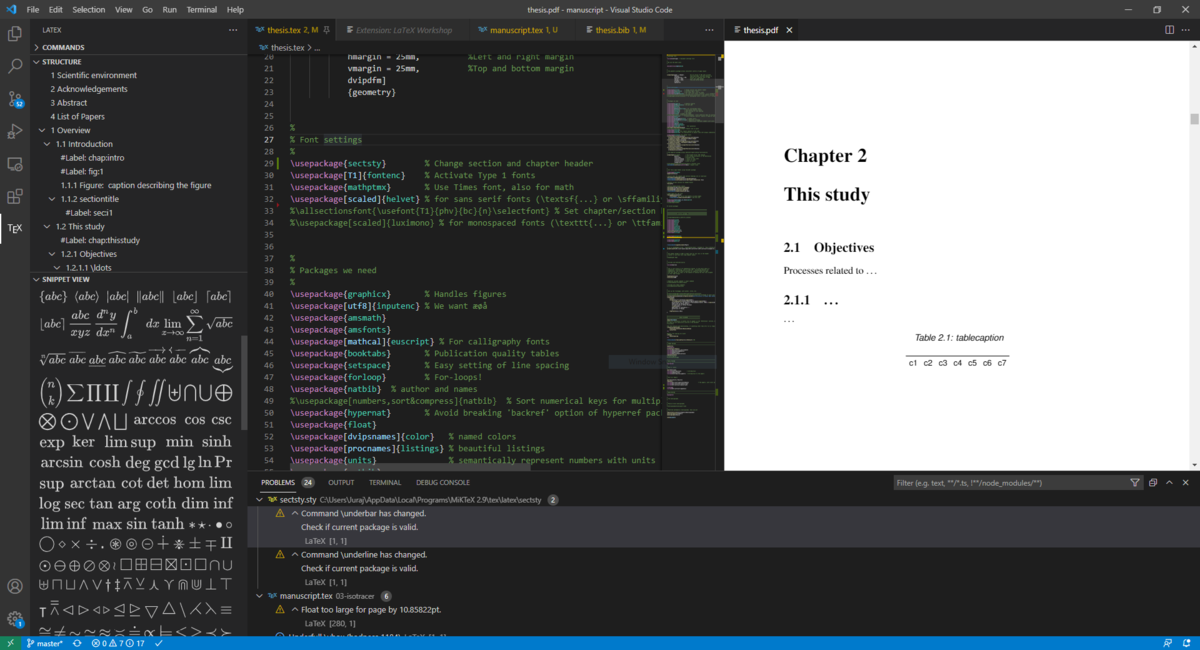
\includegraphics[width=1\columnwidth]{esempioVSCode}
    \caption{Interfaccia grafica di esempio dell'IDE Visual Studio Code.} 
    \label{fig:esempioVSCode}
    \vspace{1mm}
    Fonte: \url{https://commons.wikimedia.org/wiki/File:VsCode_LaTex_Workshop.png}.
\end{figure}
\subsubsection*{Fase 5: dal 21/10/2024 al 25/10/2024 (40h) }
Lo studente discutere con gli \emph{stakeholder} come viene utilizzato Jenkins e come è stato sponsorizzato e analizzato nei documenti di sviluppo sicuro, prendere confidenza con Jenkins realizzando un \emph{job} che compila un modulo di esempio. Lo studente determina se sia stato possibile compilare in ambito \gls{Sistemi} con l'\emph{automation server} Jenkins oppure no come descritto nei documenti di sviluppo sicuro.\\

\subsubsection*{Fase 6: dal 28/10/2024 al 31/10/2024 e dal 04/11/2024 al 08/11/2024 (72h)}
Lo studente insieme ai colleghi inserisce dei \emph{test} di esempio nel modulo e verifica di poterli eseguire con Jenkins e visionare i loro \emph{report}.\\
Verifica le possibilità di \emph{deploy} tramite Jenkins. Verifica come sia composto il \emph{server} in cui eseguire il \emph{deploy} schematizzando le sue parti insieme ai colleghi.\\

\subsubsection*{Fase 7: dal 11/11/2024 al 15/11/2024 (40h) }
Lo studente fornisce i suoi \emph{feedback} finali su quanto appreso tramite l'\emph{automation server} e sponsorizza la sua esperienza ai \emph{team} realizzando documentazione e presentazione.\\

\subsubsection*{Fase 8: dal 18/11/2024 al 20/11/2024 (24h) }
Lo studente interpreta l'esperienza per discutere di vantaggi nell'uso di un sistema di \emph{build} e \emph{deploy} automatizzato e sua sponsorizzazione in un'azienda. Ogni esperienza fatta durate lo \emph{stage} è corredata da documentazione, versionamento di configurazioni o \emph{software} se utilizzati, condivisione con gli \emph{stakeholder}.\\
Viene eseguita una presentazione finale.\\
\begin{figure}[htbp] 
    \centering 
    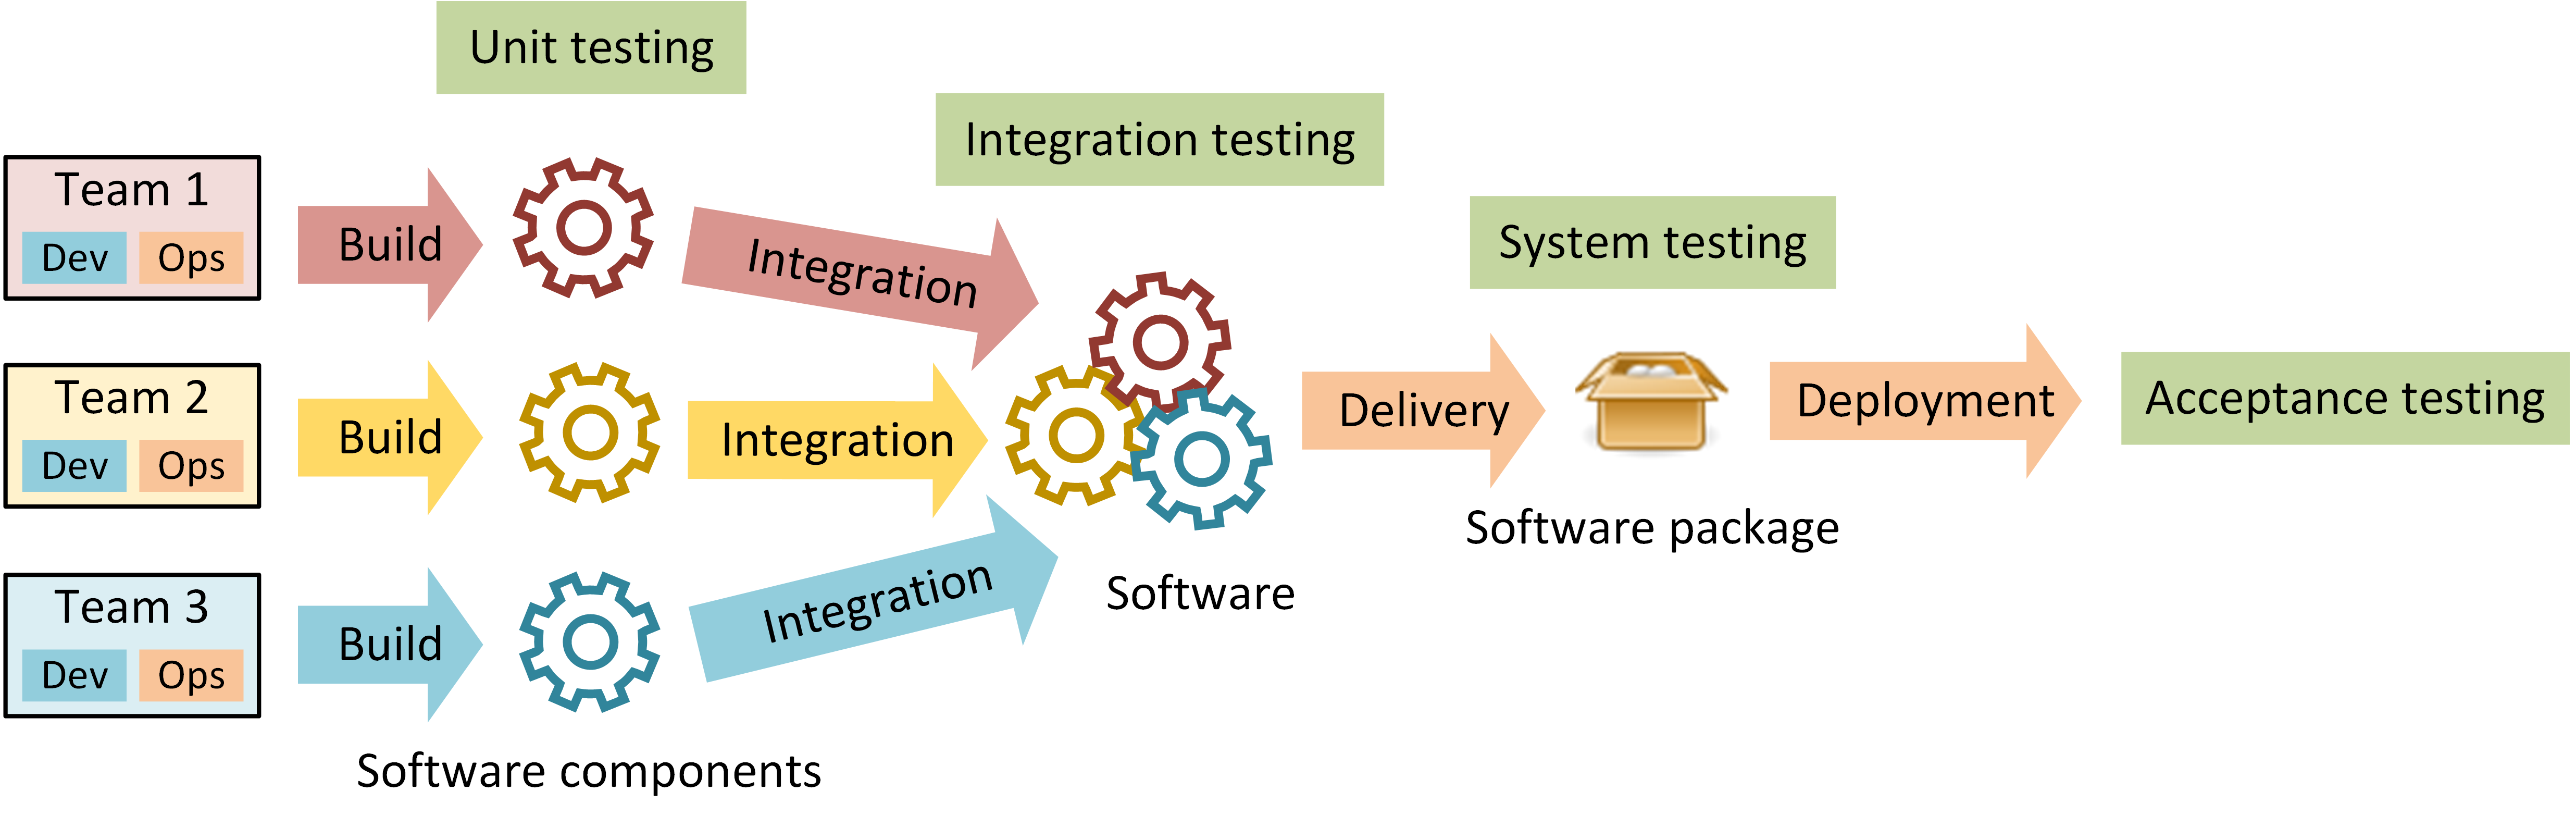
\includegraphics[width=1\columnwidth]{buildToDeployment}
    \caption{Flusso di Build, Delivery e Deployment in ambito DevOps.} 
    \label{fig:buildToDeployment}
    \vspace{1mm}
    Fonte: \url{https://commons.wikimedia.org/wiki/File:DevOps_from_Integration_to_Deployment.png}.
\end{figure}
\newline \newline \noindent Tali indicazioni sono state intese come delle linee guida e non come dei vincoli ferrei, pertanto, ho avuto la libertà di autogestire le mie attività dando priorità alle necessità e alle direttive fornitemi con l'avanzamento dei lavori.\\
Esse hanno rispettato quanto descritto con la differenza che è stata data maggiore importanza all'applicazione delle fasi di \gls{DevOps} in ambienti Office365 e allo sviluppo con le tecnologie Power Automate e Power Apps.\\\\
Inizialmente era incluso fortemente l'ambiente \gls{Sistemi} nelle fasi del progetto poiché era prevista una maggiore collaborazione con lo stage \hyperref[stageDavide]{Applicativi di \gls{DevOps} in ambito Sistemi}.\\
Questi riallineamenti sono avvenuti in maniera naturale e coerentemente con le necessità e indicazioni fornitemi dal \emph{tutor} aziendale.\\\\
Durante l'avanzamento dei lavori, le attività da me svolte sono sempre state dichiarate tramite lo strumento Planner e tutti i documenti da me realizzati sono stati condivisi in un ambiente comune al fine di mantenere chiarezza con il \emph{team} e il \emph{tutor} aziendale.\\\\
Con quest'ultimo ho potuto mantenere uno stretto contatto durante il periodo di \emph{stage} in modo da favorire l'interazione e garantire il raggiungimento degli obiettivi prefissati.\\
Ad ogni significativo risultato ottenuto ho realizzato la relativa documentazione e una presentazione successivamente esposta al \emph{tutor} e al \emph{team} di sviluppo.\\

\subsection{Obiettivi personali}
Durante l'evento STAGEIT avvenuto il giorno 8 aprile 2024, ho potuto dialogare con diverse aziende relativamente ai loro progetti di \emph{stage} offerti. Sono seguitati colloqui nelle rispettive sedi e infine ho convenuto che l'azienda che mi suscitava maggiore interesse fosse Wintech.\\
Questo è conseguenza dell'organizzazione aziendale in linea con i processi studiati durante il corso di studi, l'attenzione che è stata posta fin da subito agli stagisti e all'innovazione e grazie ai progetti di \emph{stage} relativi a tematiche di mio interesse.\\\\
È per tali motivazioni che i miei obiettivi personali sono:
\begin{itemize}
    \item Introduzione ad un contesto lavorativo, legato al percorso di studi da me frequentato, che comprendesse i principali processi aziendali studiati. 
    \item Collaborazione con un \emph{team} di sviluppo professionale utilizzando gli strumenti adeguati. 
    \item Sviluppo, analisi ed integrazione con il contesto aziendale di tecnologie per me nuove. Creazione della conseguente adeguata documentazione. 
    \item Realizzazione di flussi di automazione in grado di migliorare la produttività e la qualità dei processi aziendali e di aggiungere importanti funzionalità ad applicazioni e prodotti reali. 
    \item Gestione delle risorse e del tempo fornitomi per organizzare e realizzare in autonomia i \emph{task} definiti in fase di pianificazione.\\
\end{itemize}
Avendo deciso di non proseguire con la laurea magistrale, è rientrato maggiormente nel mio interesse entrare in un contesto lavorativo al fine di crescere professionalmente e acquisire maggiori opportunità in vista del periodo successivo al conseguimento della laurea. 

 


    \chapter{Svolgimento \emph{stage}}
\label{cap:svolgimentoStage}
In questo capitolo vengono descritte tutte le attività da me svolte durante lo \emph{stage}, divise nelle sezioni "Analisi", "Progettazione" e "Sviluppo software e documentale", in modo da fornire una panoramica chiara e strutturata del lavoro svolto, evidenziando il processo seguito e le competenze acquisite in ciascuna attività.\\
\section{Analisi}
\subsection{Requisiti}
I requisiti del mio \emph{stage}, derivanti in parte dalle dichiarazioni aziendali presenti nel documento "Progetto Formativo" generato all'inizio del suo svolgimento, e in parte conseguenza dell'analisi dei requisiti avvenuta in corrispondenza con la presenza di specifiche necessità progettuali, sono divisi in categorie:
\begin{enumerate}
	\item[O -]requisiti obbligatori, vincolanti in quanto obiettivi primari richiesti dall'azienda.
    \item[D -]requisiti desiderabili, non strettamente necessari ma dal riconoscibile valore aggiunto.
    \item[F -]requisiti facoltativi / opzionali, rappresentanti un valore aggiunto non strettamente competitivo.
\end{enumerate}

\begin{longtable}{|c|p{11cm}|}
\caption{Tabella dei requisiti progettuali.}
\label{tab:obiettiviProgettuali}\\
\hline \textbf{Codice} & \textbf{Descrizione}\\ \hline \endfirsthead
\hline \textbf{Codice} & \textbf{Descrizione}\\ \hline \endhead
\hline \endfoot
\hline \endlastfoot
\textbf{O1}    & Comprensione e mappatura delle funzionalità possibili tramite l'adozione dell'applicazione Microsoft Power Automate.\\
\hline O1.1  & Analisi approfondita riguardo ai flussi Power Automate ed individuazione delle caratteristiche, positive e negative, della sua adozione in azienda. Redazione di un documento dedicato.\\
\hline O1.2  & Sviluppo di almeno un flusso Power Automate.\\
\hline O1.3  & Produzione ed esposizione al \emph{tutor} aziendale e al \emph{team} di sviluppo di una presentazione riguardo ai risultati della mia analisi sull'adozione di Power Automate in azienda.\\
\hline \textbf{O2}  & Comprensione ed utilizzo della tecnologia Microsoft Power Apps e relative fasi di sviluppo collaborativo.\\
\hline O2.1  & Comprensione di Power Apps mediante lo svolgimento di attività di affiancamento con il \emph{team} di sviluppo fino al raggiungimento della comprensione dei metodi lavorativi e dei prodotti aziendali sviluppati con tale strumento.\\
\hline O2.2  & Identificazione e utilizzo di un metodo adatto allo sviluppo collaborativo di applicazioni Power Apps.\\
\hline O2.3  & Ottenimento di avanzamenti nello stato dei lavori di applicazioni aziendali realizzate con Power Apps.\\
\hline \textbf{O3}  & Individuazione ed implementazione di un efficace sistema di versionamento per progetti realizzati utilizzando tecnologie Power Automate e Power Apps\\
\hline \textbf{O4}  & Comprensione delle metodologie \gls{DevOps} e realizzazione della documentazione relativa alla sua applicabilità su tecnologie Power Automate e Power Apps.\\
\hline 
\hline \textbf{D1}  & Collaborazione con gli altri stagisti universitari e individuazione di soluzioni collaborative relative ai bisogni progettuali comuni.\\
\hline \textbf{D2}  & Realizzazione di PoC a supporto delle soluzioni individuate durante le fasi di ricerca.\\
\hline D2.1  & Realizzazione di PoC riguardo allo sviluppo di flussi Power Automate approvativi.\\
\hline D2.2  & Realizzazione di PoC riguardo all'integrazione tra flussi Power Automate ed elementi esterni tramite le chiamate \gls{http}.\\
\hline D2.3  & Realizzazione di PoC riguardo al processo \gls{DevOps} di \emph{build} su progetti realizzati con tecnologie Power Automate/Power Apps.\\
\hline D2.4  & Realizzazione di PoC riguardo al processo \gls{DevOps} di \emph{test} su progetti realizzati con tecnologie Power Automate/Power Apps.\\
\hline \textbf{D3}  & Esecuzione di \emph{meeting} e scambio di documenti con gli altri stagisti universitari al fine di comprendere l'applicabilità delle fasi di \gls{DevOps} in ambito \gls{Sistemi} \\
\hline 
\hline \textbf{F1}  & Esplorazione della tecnologia Angular mediante realizzazione di un progetto di \emph{test}\\
\hline \textbf{F2}  & Integrazione di un progetto Angular con le fasi di \gls{DevOps} mediante un \emph{server} Jenkins.\\
\hline \textbf{F3}  & Realizzazione ed esposizione di una presentazione finale, in collaborazione con gli altri stagisti, riguardo tutto il lavoro fatto durante lo \emph{stage}.\\
\end{longtable}

\subsection{Ambiente di lavoro}
Durante i primi giorni dello \emph{stage} sono stato introdotto all'ambiente di lavoro e alle tecnologie di comunicazione e collaborazione utilizzate.\\
Conseguentemente ho analizzato e utilizzato il sistema di messaggistica basato su Microsoft Teams e Outlook e ho compreso la struttura di condivisione dei dati, utilizzata in azienda, basata sullo strumento Microsoft SharePoint.
Esso è una piattaforma \emph{software} in grado di organizzare dati sottoforma di \emph{file} e strutture tabellari chiamate "Liste", al fine di gestire il materiale condiviso dall'azienda e dai singoli \emph{team} tramite un sistema di accessi e autorizzazioni.\\
Tramite questi strumenti ho studiato i documenti aziendali a me forniti in modo da comprendere i principali processi produttivi di Wintech.\\ 
Tali documenti comprendono i "Documenti di sviluppo sicuro" e includono:
\begin{itemize}
    \item Agile e SCRUM: descrizione delle metodologie Agile e SCRUM, spiegazione dei ruoli necessari e delle cerimonie previste. 
    \item Presentazione sviluppo sicuro: presentazione PowerPoint che descrive i processi aziendali atti a migliorare la qualità dei prodotti realizzati automatizzando fasi ripetitive e rispettando criteri di sicurezza. 
    \item Modelli di sviluppo sicuro: elenco dettagliato dei documenti di sviluppo sicuro i quali descrivono come applicare automazioni processuali (per esempio i processi di \emph{build} e \emph{deploy}) in modo sicuro e normato. 
    \item Politiche di sviluppo sicuro: strategie e normative aziendali definite al fine di garantire sicurezza e qualità nei processi e nel ciclo di vita del \emph{software}. 
    \item Piani di progetto degli altri stagisti: piani formativi degli altri due stagisti che nel mio stesso periodo hanno effettuato lo \emph{stage} universitario in Wintech. 
\end{itemize}
Relativamente a quest'ultimo punto, nei primi giorni ho approfondito il lavoro svolto dagli altri stagisti tramite appositi \emph{meeting} nei quali mi hanno descritto i risultati ottenuti fino a quel momento. Essi, avendo iniziato lo svolgimento del progetto circa una settimana prima, mi hanno esposto, mediante apposite presentazioni PowerPoint, le proprie ricerche riguardanti l'utilizzo dello strumento Git e dello studio avvenuto riguardo la possibilità di integrare tra loro gli strumenti Planner e Taiga. 

\subsection{Tecnologie oggetto di \emph{stage}}
Questa sottosezione descirve i metodi di apprendimento e le nozioni apprese durante la fase di analisi delle tecnologie su cui si basa la ricerca del mio progetto di \emph{stage}.\\
Dopo aver compreso le tecnologie e i principali processi aziendali, ho partecipato ad un \emph{meeting} con il \emph{tutor} aziendale al fine di discutere il mio progetto di \emph{stage}.\\
Gli obiettivi scaturiti da tale incontro sono stati: 
\begin{itemize}
    \item Autoapprendimento dello strumento Power Automate.
    \item Realizzazione di un PoC che testasse la possibilità di realizzare un flusso approvativo Power Automate. 
    \item Testare le funzionalità disponibili con le licenze di utilizzo \emph{standard}. 
\end{itemize}

\subsubsection*{Power Automate}
Ho pertanto studiato approfonditamente tali tecnologie con l'ausilio delle numerose guide e \emph{tutorial} offerti da Microsoft. 
Essi sono direttamente accessibili dalla \emph{home} di Power Automate e Power Apps e sono divisi in moduli testuali corredati da immagini, dalla durata e argomenti specifici. 

\begin{figure}[htbp] 
    \centering 
    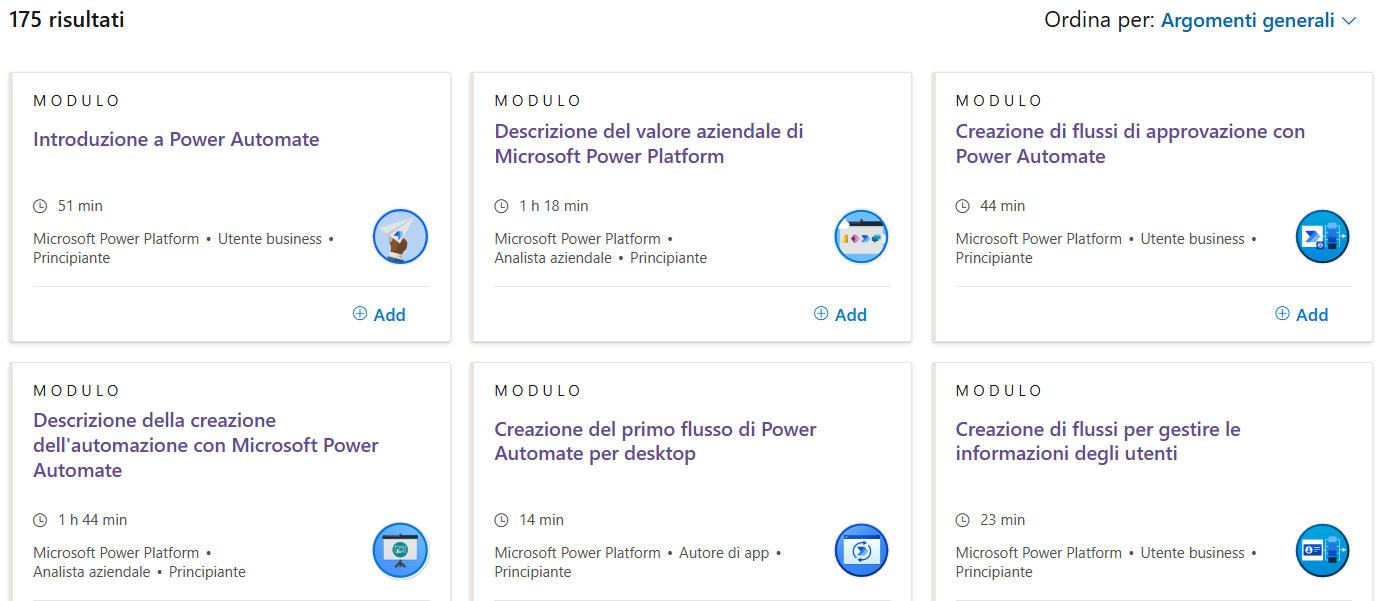
\includegraphics[width=1\columnwidth]{moduliPowerAutomate} 
    \caption{Moduli formativi per Power Automate.}
    \label{fig:moduliPowerAutomate}
    \vspace{1mm}
    Fonte: \url{https://learn.microsoft.com/it-it/training/browse/?products=power-automate}.
\end{figure}

\noindent Lo studio di tali moduli mi ha permesso di comprendere il funzionamento e le \emph{features} principali di Power Automate.
Esso è formato da una pagina \emph{web} che offre controllo sui flussi di automazione creati: è possibile modificarli e visualizzarne i dettagli, le esecuzioni e le statistiche. Inoltre, si possono creare dei nuovi flussi partendo da altri progetti pubblici, o a noi condivisi, e modelli offerti da Microsoft da adattare alle proprie esigenze.\\
La modifica di un flusso non avviene mediante la scrittura di codice tramite un linguaggio di programmazione, bensì tramite una composizione "a blocchi" personalizzabili collegati tra loro ciascuno avente proprietà e attributi definiti.\\
Essi sono selezionabili da una lista di blocchi relativi ciascuno a una funzionalità specifica di un servizio Microsoft.
Tali blocchi possono essere "Trigger" o "Azioni" ed entrambi sono necessari per la creazione e il funzionamento di un flusso.
In ogni flusso è presente uno e un solo Trigger il quale rappresenta il suo punto di partenza nonché la condizione che scaturisce la sua esecuzione.\\
Esistono tre tipologie principali di Trigger le quali determinano la tipologia stessa di ogni flusso:
\begin{itemize}
    \item Automatico: per esempio "SharePoint - Quando viene creato un elemento". 
    \item Istantaneo: per esempio "Attiva manualmente un flusso".
    \item Pianificato: per esempio "Ricorrenza", il quale attiva il flusso periodicamente.\\
\end{itemize}

\noindent Ad ogni Trigger possono essere collegate, in serie o in parallelo, una moltitudine di Azioni, ciascuna responsabile di uno specifico compito, per esempio sono presenti le azioni "Inizializza variabile", "Avvia e attendi un'approvazione", "Teams - Crea una chat" e "Outlook - Invia un messaggio di posta elettronica".\\
Sono inoltre presenti azioni dedicate alla gestione logica dei flussi come "Condizione" e "Do until". La prima rappresenta la struttura di controllo rappresentata nei classici linguaggi di programmazione con "if", responsabile della ramificazione dell'esecuzione del flusso in base a una condizione specifica.
La seconda rappresenta la struttura di controllo rappresentata nei classici linguaggi di programmazione con "Do while", responsabile della ripetizione condizionata di un insieme di azioni garantendone sempre la prima esecuzione.
\begin{figure}[htbp] 
    \centering 
    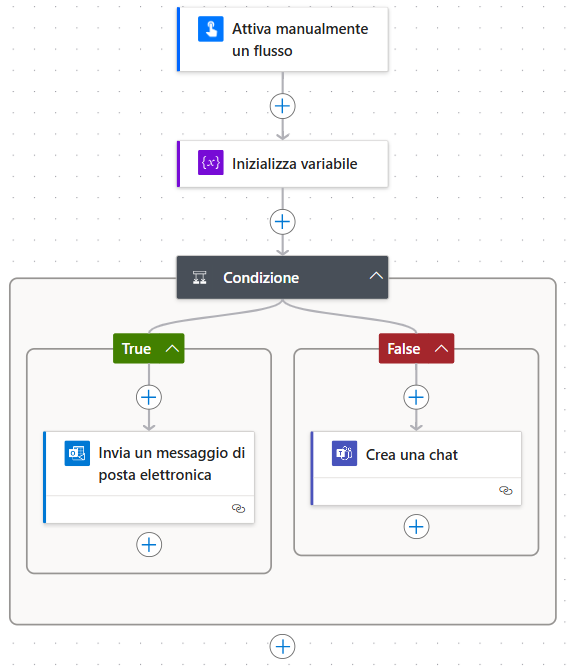
\includegraphics[width=0.6\columnwidth]{esempioFlusso} 
    \caption{Esempio di un flusso Power Automate istantaneo.}
    \label{fig:esempioFlusso}
\end{figure}
\newline \noindent Successivamente ho individuato, durante un meeting con il \emph{tutor} aziendale, la necessità di integrare i flussi Power Automate con il \emph{software} gestionale \hyperref[WOW]{WOW} e gli altri prodotti aziendali, al fine di poter integrare le funzionalità desiderate con libertà mantenendo coordinate le diverse parti del prodotto.\\
Sono emersi quindi due requisiti: il primo, utile per apprendere le tecnologie in oggetto, è relativo alla creazione di un flusso che automatizzi un processo approvativo (requisito D2.1).\\
Il secondo (requisito D2.2), più concreto e integrabile con i prodotti aziendali, si focalizza sull'applicazione ai flussi Power Automate di chiamate \gls{http}(Hypertext Transfer Protocol): in italiano "protocollo di trasferimento ipertestuale", è un protocollo di rete, ovvero un insieme di regole formalmente descritte che definiscono le modalità di comunicazione tra due o più apparecchiature elettroniche, usato come principale sistema per la trasmissione di informazioni sul \emph{web}.
\subsubsection*{Power Apps}
I flussi Power Automate portano grande vantaggio in termini di efficienza dei processi aziendali e possono aumentare il numero di funzionalità di un'applicazione.\\
Per questo motivo il loro utilizzo assume maggiore significato quando associato alla realizzazione di applicazioni Power Apps, le quali sono pensate per integrare nativamente i flussi creati.\\
Il metodo di apprendimento con cui ho analizzato e studiato Power Apps deriva non solo da attività individuali tramite i moduli didattici offerti da Microsoft nell'apposito sito \emph{web}, simili a quelli per Power Automate, ma soprattutto grazie alla collaborazione con un membro del \emph{team} di sviluppo che ho affiancato.\\
Egli è il responsabile in azienda di tutti i loro prodotti realizzati utilizzando le tecnologie oggetto del mio \emph{stage}, e assieme le abbiamo attentamente analizzate e modificate al fine di migliorarle ed applicarci le soluzioni da me individuate relativamente alle pratiche \gls{DevOps} richieste.\\
Power Apps offre la possibilità di creare nuove applicazioni e visionare quelle già create, o a noi condivise, con la possibilità di apportare modifiche.\\
È inoltre possibile visualizzare informazioni e statistiche relative a tutte le applicazioni in nostro possesso.\\
Il loro sviluppo non avviene esclusivamente mediante codice di programmazione bensì dall'utilizzo di componenti, \emph{standard} o \emph{custom}, che vengono manualmente posizionati sull'interfaccia, creando in questo modo una struttura gerarchica ad albero chiamata "Tree View".
\begin{figure}[htbp] 
    \centering 
    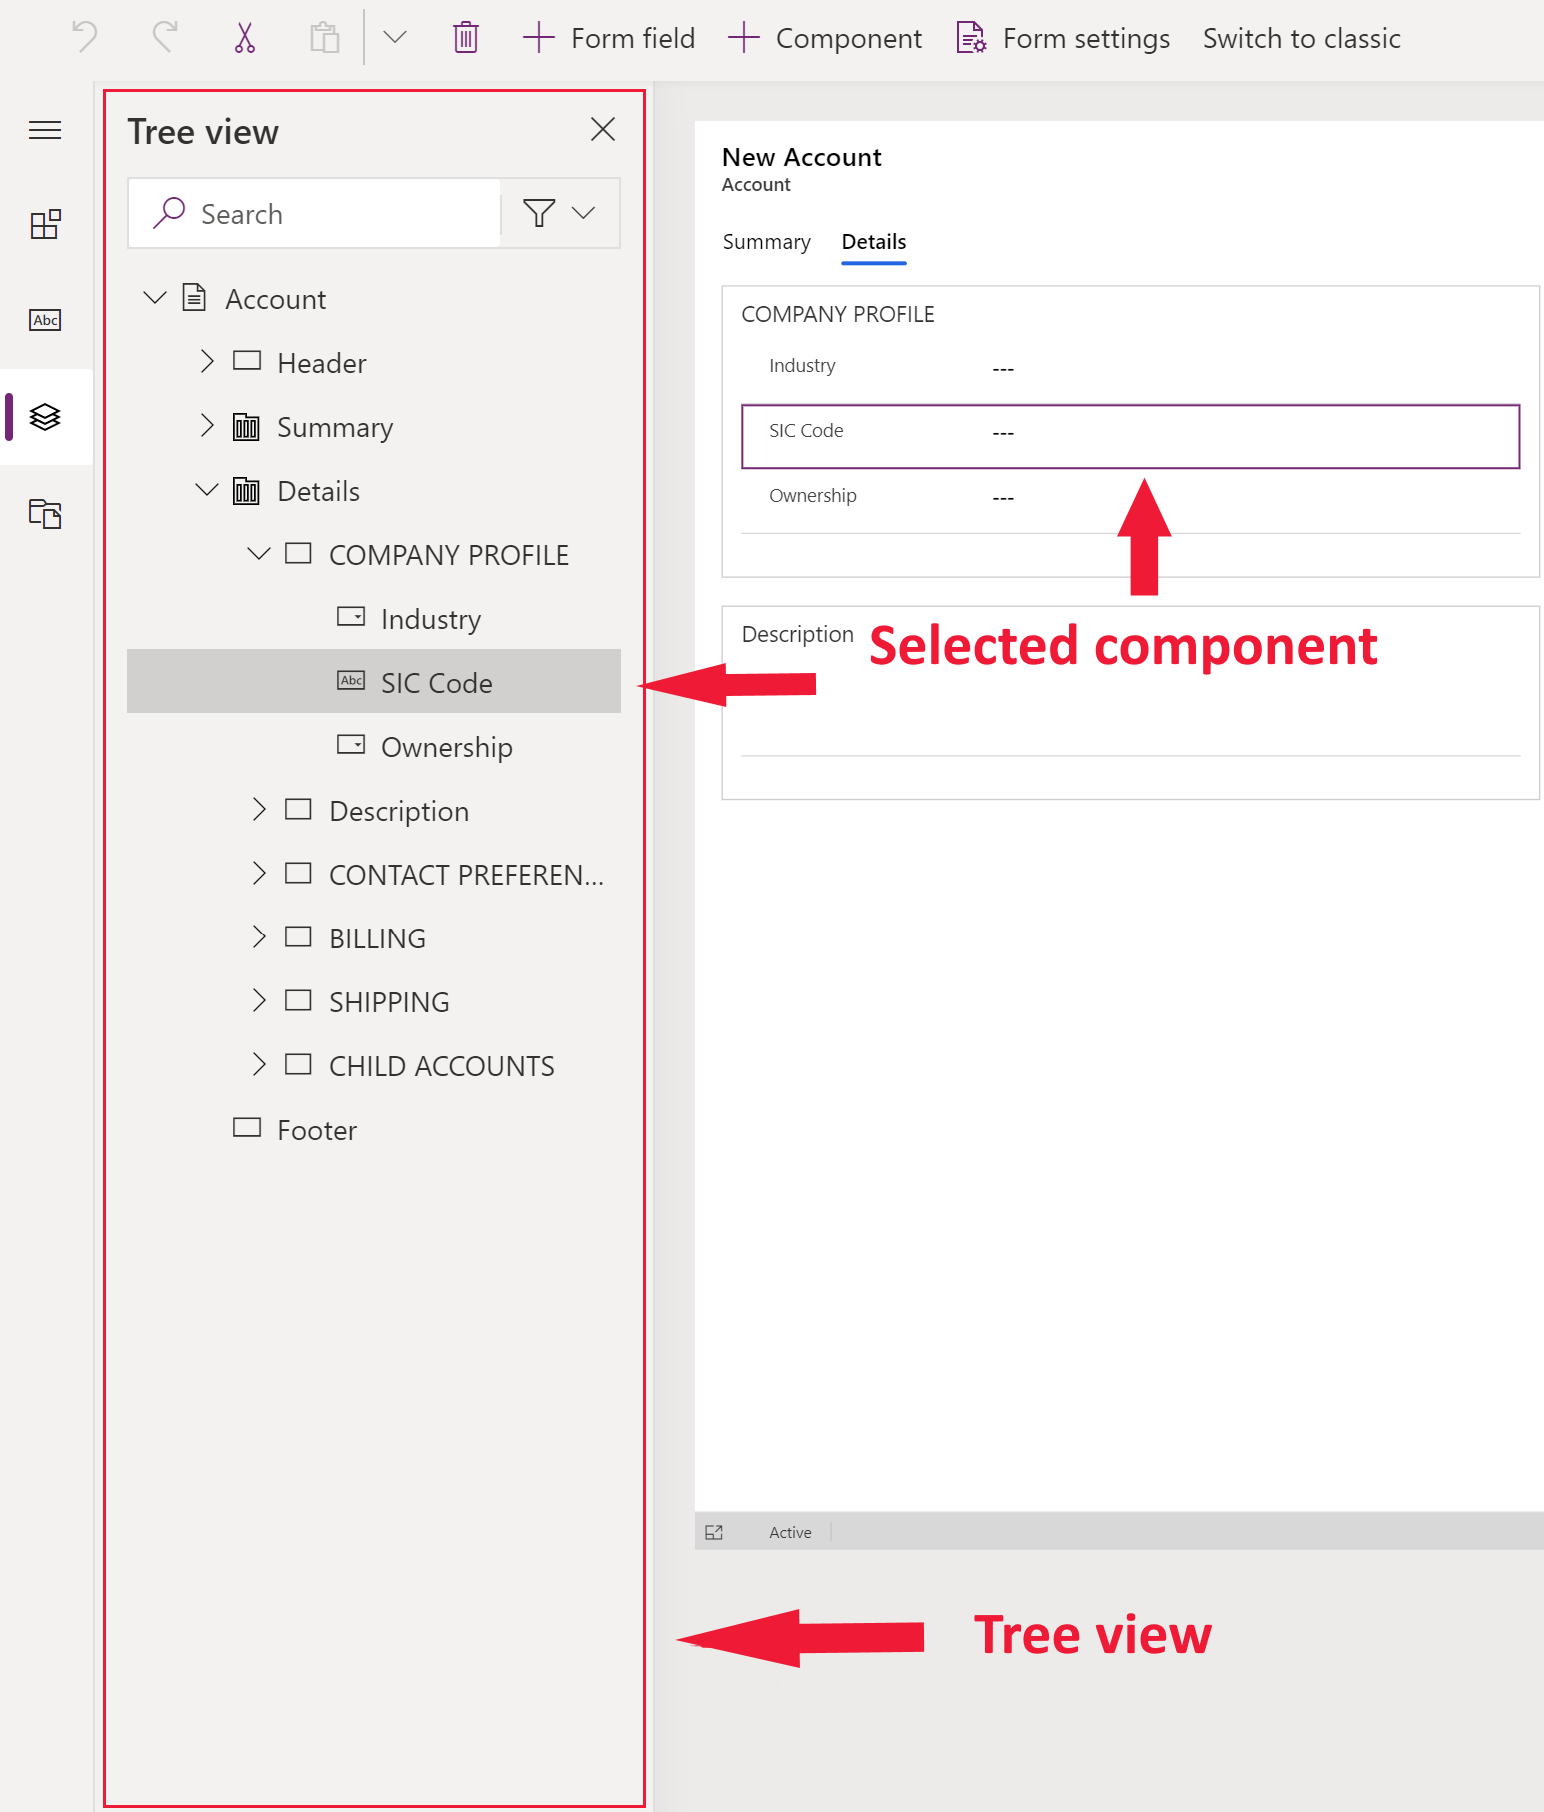
\includegraphics[width=0.6\columnwidth]{powerAppsTreeView} 
    \caption{Elemento Tree View per la gestione gerarchica dei componenti.}
    \label{fig:powerAppsTreeView}
    \vspace{1mm}
    Fonte: \url{https://learn.microsoft.com/en-us/power-apps/maker/model-driven-apps/using-tree-view-on-form}.
\end{figure}
\newline \noindent Al fine di modificare i parametri che lo compongono, ciascun componente può essere personalizzato tramite un'apposita finestra dell'interfaccia grafica.\\
Questo non comprende solo le peculiarità grafiche ma soprattutto il loro comportamento a seguito di azioni specifiche: per esempio è possibile creare un componente "Pulsante" e personalizzarne il campo "OnSelect" al fine di eseguire conseguentemente un flusso Power Automate e inviarne i dati di \emph{output} ad un altro componente.\\
Tali istruzioni vengono definite utilizzando Microsoft Power Fx, il quale rappresenta un linguaggio di programmazione dichiarativo, fortemente tipizzato e con uso limitato di codice, usato in Microsoft Power Platform.\\
Quest'ultima piattaforma include un insieme di strumenti e tecnologie, compresi Power Automate e Power Apps, pensati per offrire la possibilità di sviluppare prodotti \emph{software} con limitata necessità di scrivere, e conoscere, codice tramite linguaggi di programmazione.\\\\

\subsection{Tecnologie di supporto}
\subsubsection*{Jenkins}
Al fine di applicare le automazioni necessarie per adottare al \emph{software} le metodologie \gls{DevOps}, come richiesto dagli obiettivi di \emph{stage}, ho individuato lo strumento Jenkins in quanto esso rispecchia perfettamente le mie necessità ed è inoltre già conosciuto e applicato dal resto del \emph{team} di sviluppo, rappresentando quindi una tecnologia consolidata che non necessita di ulteriore formazione all'interno dell'azienda.\\
Ho appreso le conoscenze necessarie per studiare e utilizzare tale strumento in totale autonomia mediante la consultazione delle guide e del numeroso materiale presente \emph{online} comprese le pagine \emph{web} ufficiali di Jenkins con gli annessi video \emph{tutorial}.\\
Esso è uno strumento scritto in linguaggio di programmazione Java che viene eseguito all'interno di un \emph{web server} e offre la possibilità di creare, gestire, eseguire e monitorare dei progetti Jenkins chiamati "Job", potendone visionare e registrare i \emph{report} di \emph{output}.\\
Essi sono unità di lavoro configurabili che rappresentano un'attività o un progetto specifico che Jenkins esegue. Inoltre possono essere di diverso tipo ma tutti sono basati sull'esecuzione di uno \emph{script} o una \emph{pipeline} di automazione.\\
Una \emph{pipeline} Jenkins è una sequenza di fasi chiamate "Stage", eseguite in serie o in parallelo, responsabili di specifiche operazioni definite dall'utente, per esempio \emph{build}, \emph{test}, \emph{deploy}.\\
Esse possono essere definite tramite il linguaggio di programmazione Groovy oppure tramite l'interfaccia grafica di Jenkins.\\
Questo strumento permette dunque di fornire servizi di integrazione continua ed è indicato per l'applicazione di alcune fasi di \gls{DevOps} come Build e Test, il caricamento automatico dei \emph{file} sul \emph{repository} di versionamento desiderato e l'autenticazione automatica ai servizi Microsoft tramite comandi Power Platform CLI.\\
Quest'ultima è un'interfaccia a riga di comando che offre la possibiltà di eseguire un insieme di comandi specifici atti all'autenticazione e alla gestione degli ambienti e delle Microsoft Solutions.\\
\begin{figure}[htbp] 
    \centering 
    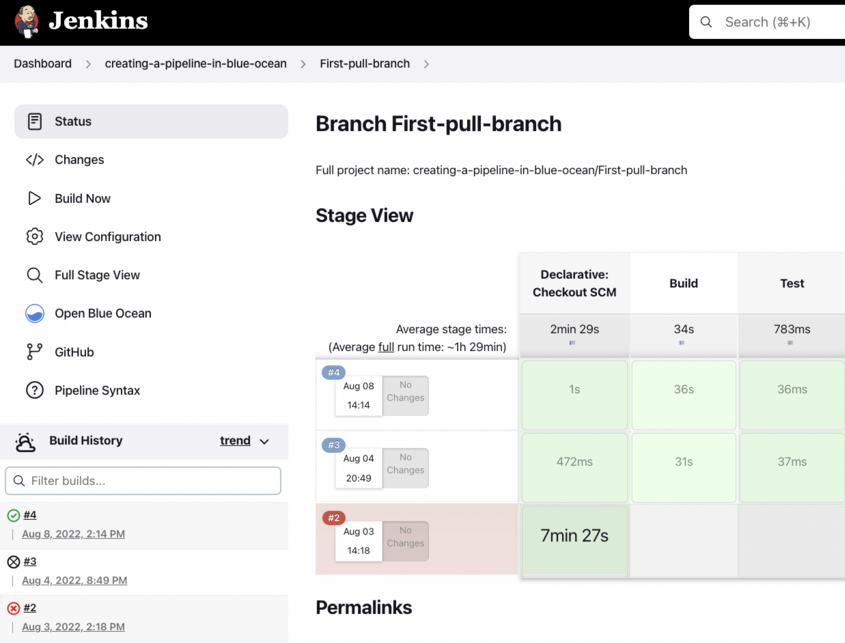
\includegraphics[width=0.9\columnwidth]{esempioJenkins} 
    \caption{Esempio interfaccia di Jenkins.}
    \label{fig:esempioJenkins}
    \vspace{1mm}
    Fonte: \url{https://commons.wikimedia.org/wiki/File:Updated-jenkins-view.png}.
\end{figure}

\newpage \subsubsection*{Microsoft Solutions}
Un'ulteriore oggetto di analisi e studio è stato l'utilizzo e la comprensione delle Microsoft Solutions. Esse fanno parte della \emph{suite} Microsoft Power Platform e sono degli strumenti che servono a contenere tutti i flussi Power Automate e applicazioni Power Apps corrispondenti a uno stesso progetto, in modo da poterli sviluppare e distribuire in maniera organizzata e centralizzata.\\
Esistono due tipi di Soluzioni: 
\begin{itemize}
    \item Gestite: destinate prevalentemente per gli ambienti di produzione e \emph{test}, non permettono la modifica degli elementi al suo interno. Per generare una Soluzione gestita è necessario esportare una soluzione non gestita.
    \item Non gestite: destinate prevalentemente per gli ambienti di sviluppo, permettono la modifica degli elementi al suo interno e la sua esportazione.
\end{itemize}
A differenza delle tecnologie precedentemente descritte, le Microsoft Solution non erano materia già affrontata in azienda, per cui il loro apprendimento è avvenuto in maniera totalmente autonoma mediante la documentazione presente nei siti \emph{web} Microsoft dedicati.\\
Le Soluzioni preservano i loro dati, e quelli degli elementi in esse contenuti, nel sistema di archiviazione Microsoft Dataverse che funge da \emph{database} centralizzato per applicazioni sviluppate con la Power Platform.\\
Tale adozione permette di usufruire di funzionalità altrimenti assenti.
Le conseguenze del loro utilizzo e le motivazioni che mi hanno portato ad utilizzare questa tecnologia sono materia di discussione presente nella sezione \hyperref[progettazioneSolutions]{Adozione delle Microsoft Solutions}.\\

\subsection{DevOps}
Prima di poter progettare una soluzione applicativa al fine di applicare le fasi di \gls{DevOps} a progetti realizzati con Power Automate e Power Apps, ho analizzato e compreso quali fossero le implicazioni di ogni \emph{step}.\\
Ho approfondito tale pratica soprattutto studiando gli approfondimenti presenti sul sito \emph{web} di Atlassian, nota compagnia di \emph{software enterprise}, e dalla teoria sul ciclo di vita del \emph{software} e sulle metodologie di automazione dei processi aziendali appresa durante il percorso di studi universitario.\\
Ho inoltre studiato i documenti di sviluppo sicuro aziendali, nei quali sono presenti delle linee guida su come adottare il \gls{DevOps} in Wintech.\\
Le sue fasi sono:
\subsubsection*{Plan}
Essendo la fase iniziale del ciclo, ha lo scopo di definire i requisiti, pianificare il ciclo di vita del progetto e identificarne le metodologie di lavoro. Adottando una metodologa iterativa, è consono che la pianificazione e le conseguenti fasi successive, possano subire modifiche rispetto alle precedenti pianificazioni.

\subsubsection*{Code}
Dopo aver compreso cosa e come soddisfare i requisiti progettuali, vengono sviluppate le soluzioni individuate seguendo le metodologie e le norme definite in fase Plan.\\
Essendo il progetto di \emph{stage} basato su tecnologie non sviluppabili tramite strumenti tradizionali, come IDE non proprietari e linguaggi di programmazione consolidati, l'analisi della fase Code è stata necessaria per comprendere le funzionalità disponibili agli utenti al fine di sviluppare tali prodotti.\\
È compresa in questa fase anche la ricerca avvenuta al fine di individuare le metodologie e gli strumenti adatti a sviluppare progetti con le tecnologie in oggetto in maniera collaborativa e adottando un efficace metodo di versionamento.\\
Questo ha necessitato di uno studio sullo strumento Git, già ampiamente affrontato durante il percorso di studi universitari.\\
Infine, è compresa nella fase Code anche l'attività di analisi statica del codice, la quale supporta le fasi di sviluppo identificando e segnalando eventuali errori nel codice sorgente senza la necessità di eseguirlo.

\subsubsection*{Build}
Fase relativa alla creazione dei pacchetti e dei \emph{file} eseguibili costruiti partendo dal codice sorgente prodotto nella fase precedente.\\
Il risultato di questa operazione rappresenta il prodotto sul quale verranno effettuati i \emph{test} e le verifiche necessarie. 

\subsubsection*{Test}
Ottenuto l'artefatto generato dalla fase Build, esso può essere testato mediante l'utilizzo di svariati strumenti appositi.\\
Essi comprendono diversi tipi di \emph{test} dinamici: 
\begin{itemize}
    \item Test di unità: verifica che le singole unità di codice, per esempio funzioni, metodi o classi, funzionino come previsto.
    \item Test di integrazione: verifica che più parti di codice o servizi interagiscano tra loro correttamente.
    \item Test di carico: verifica il comportamento del sistema sotto carico normale ed elevato.
    \item Test di sicurezza: individua le eventuali vulnerabilità o minacce di sicurezza presenti nel sistema. 
\end{itemize}
Durante le fasi analitiche del mio \emph{stage}, ha avuto molta rilevanza lo studio sui metodi nativi ed esterni applicabili ai flussi Power Automate e alle applicazioni Power Apps al fine di applicare \emph{test}. 

\subsubsection*{Release}
Quando il prodotto è stato creato e testato, esso è considerato pronto per essere reso disponibile ai clienti, e viene quindi rilasciato identificandone una versione specifica.

\subsubsection*{Deploy}
Una versione rilasciata del prodotto viene distribuita nello specifico ambiente di produzione in cui gli utenti finali lo utilizzeranno, garantendone il corretto funzionamento.

\subsubsection*{Operate}
La gestione e il funzionamento dell'applicazione in produzione viene garantita tramite attività come l'amministrazione e la manutenzione dei \emph{server} e la risoluzione dei problemi. 

\subsubsection*{Monitor}
Al fine di garantire affidabilità e buone prestazioni del sistema distribuito, il suo comportamento viene osservato tramite strumenti che ne raccolgono e analizzano i dati. 
Vengono inoltre raccolti i \emph{feedback} degli utenti finali e dei clienti al fine di migliorare la qualità del prodotto. 

\subsection{Analisi delle applicazioni aziendali}
Il \emph{focus} principale dello \emph{stage} è compiere un'analisi sulle tecnologie al fine di raggiungere gli obiettivi riguardanti la ricerca sull'effettiva applicabilità delle pratiche di \gls{DevOps} ai progetti realizzati con Power Automate e Power Apps.
È stato però fin da subito definito che avrei alternato tali attività con fasi di sviluppo su applicazioni aziendali al fine di approfondire la conoscenza delle tecnologie in oggetto e di diventare operativo in modo più efficace.\\
Insieme al membro del \emph{team} di sviluppo responsabile per la realizzazione delle applicazioni Power Apps e dei flussi Power Automate aziendali, ho affrontato problemi di sviluppo di vario genere in funzione delle necessità del momento, potendo analizzare diversi prodotti aziendali.\\
Le effettive attività di programmazione svolte su queste applicazioni sono presenti nella sezione \hyperref[sviluppoApplicazioni]{Sviluppo di applicazioni aziendali}.\\
I principali prodotti su cui abbiamo collaborativamente lavorato sono:
\subsubsection*{Report di visita}
Principale applicazione su cui ho lavorato e con cui ho svolto attività di analisi al fine di comprendere le tecnologie utilizzate. Essa ha l'obiettivo di offrire la possibilità ad un dipendente dell'azienda, il quale dovesse trovarsi nella sede di un cliente, di registrare e condividere con i colleghi, in un ambiente condiviso, un \emph{report} della visita al fine di tracciare l'esperienza con il cliente.\\
Essa offre quindi la possibilità di: 
\begin{itemize}
    \item Ricercare e selezionare una specifica azienda visualizzabile in un'apposita lista a schermo 
    \item Visualizzare le sedi e le filiali dell'azienda selezionata 
    \item Visualizzare le informazioni anagrafiche dei contatti dell'azienda selezionata  
    \item Visualizzare i \emph{report} di visita già creati come bozza  
    \item Modificare eventuali bozze selezionate 
    \item Creare un nuovo documento inserendo in un apposito \emph{form} i dati relativi all'operatore, al cliente e alla visita specifica 
    \item Salvare tale \emph{report} come bozza o come documento definitivo
    \item Caricare automaticamente i dati generati nel \emph{database} aziendale 
\end{itemize}
\begin{figure}[htbp] 
    \centering 
    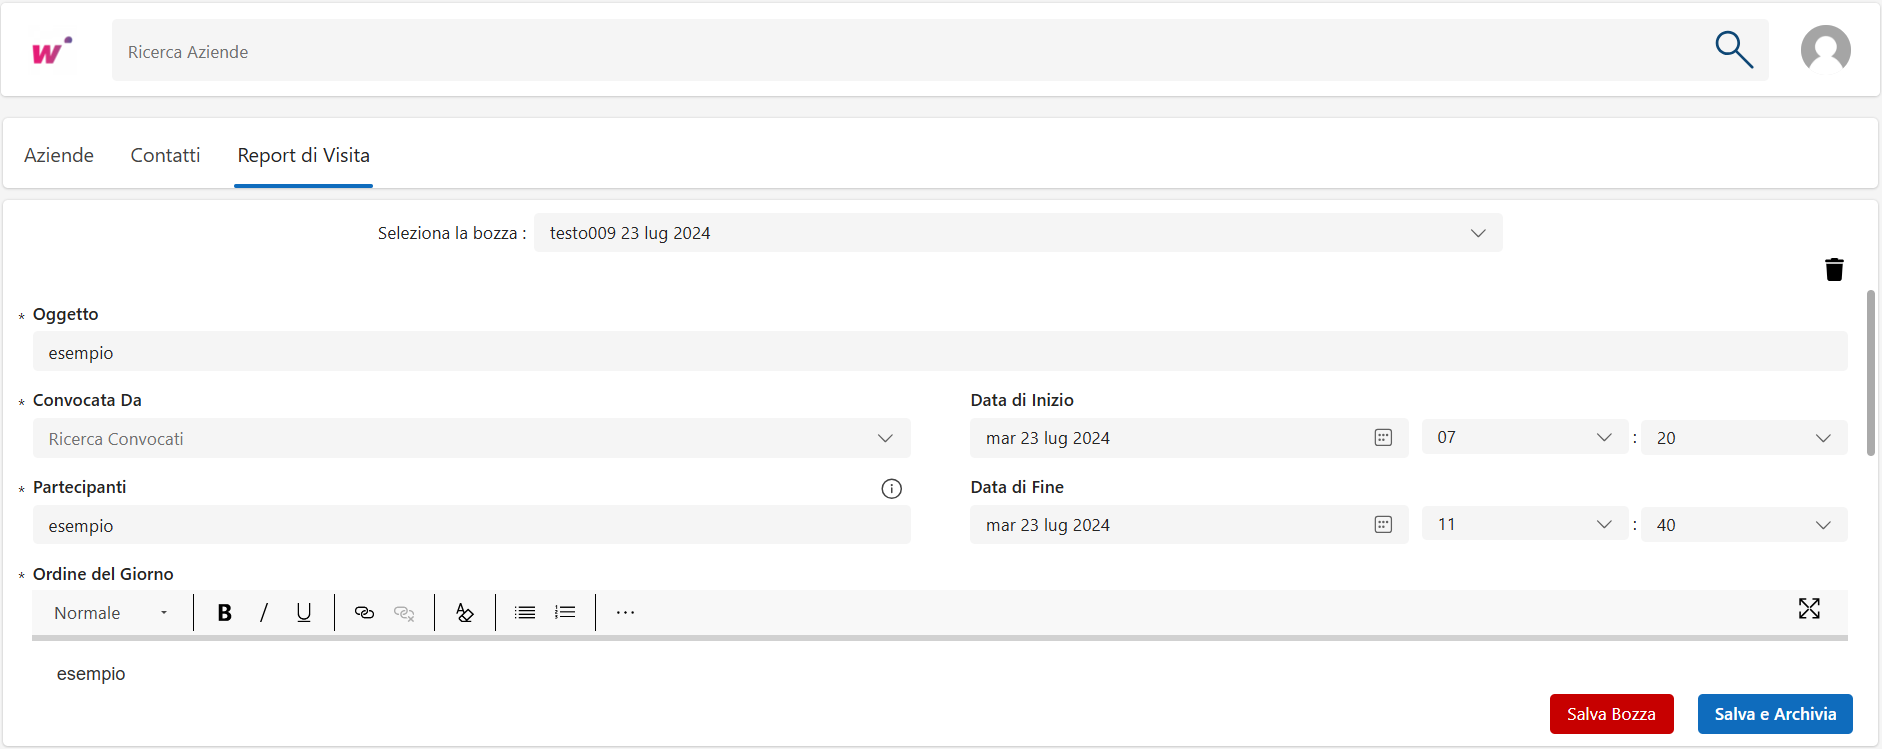
\includegraphics[width=1\columnwidth]{RDV} 
    \caption{Interfaccia grafica di Report di visita.}
    \label{fig:RDV}
\end{figure}

\subsubsection*{Registro accessi}
Applicazione realizzata al fine di gestire agevolmente i \emph{check-in} e \emph{check-out} lavorativi del personale.\\
Le funzionalità presenti sono: 
\begin{itemize}
    \item Identificazione del dipendente
    \item Selezione della sede, compresa la possibilità di selezionare lo \emph{smart working} o lavoro fuorisede 
    \item Selezione del \emph{check-in} 
    \item Visualizzazione di errore in caso di \emph{check-in} in mancanza del precedente \emph{check-out} 
    \item Selezione del \emph{check-out} 
    \item Visualizzazione di errore in caso di \emph{check-out} in mancanza del precedente \emph{check-in} 
    \item Visualizzazione di tutti i propri \emph{check-in} e \emph{check-out} 
\end{itemize}

\subsubsection*{Non conformità}
Nel momento in cui ho svolto lo \emph{stage}, questa applicazione era nelle sue prime fasi di sviluppo e le sue funzionalità non erano state ancora definite pienamente.\\
I suoi obiettivi sono quelli di creare e gestire un flusso approvativo a più \emph{step}, dove per ogni fase vengono notificati i corrispondenti incaricati, ai quali viene richiesta la compilazione di \emph{form} relativi alla non conformità di un prodotto e alle conseguenti azioni da intraprendere.\\

\subsection{Angular}
Gli ultimi requisiti emersi durante lo svolgimento dello \emph{stage} sono quelli relativi allo studio e all'applicazione di alcune fasi di \gls{DevOps} a progetti realizzati con lo strumento Angular.\\
Esso è un \emph{framework} per la realizzazione di applicazioni \emph{web} tramite il linguaggio di programmazione TypeScript e rappresenta una delle principali tecnologie usate dai \emph{team} di sviluppo di Wintech.\\
È per questo motivo che, nel momento in cui ho terminato le attività previste per il mio \emph{stage} con alcuni giorni di anticipo, mi è stato affidato il compito di studiare e provare ad utilizzare le stesse loro tecnologie e metodologie di lavoro al fine di comprenderle al meglio ed integrarmi maggiormente nell'ambiente lavorativo.\\
Tramite il sito \emph{web} ufficiale di Angular, ho seguito le guide fornite in modo da apprenderne le basi e poter realizzare quanto richiesto soddisfacendo i requisiti assegnati.\\

\section{Progettazione}
%In questa sezione sono presenti tutte le attività di progettazione da me svolte e il suo scopo è descrivere le modalità con cui ho individuato le soluzioni ai bisogni progettuali in modo da soddisfarne i requisiti.
\subsection{\emph{Scope} di Power Automate e Power Apps}
A seguito dell'analisi avvenuta sulle tecnologie oggetto di \emph{stage} è stato possibile identificare il compito che Power Automate e Power Apps devono avere all'interno di un progetto. 
Esse sono infatti tecnologie pensate per sviluppare in maniera rapida soluzioni relativamente semplici. Nel momento in cui ci fosse la necessità di applicare logiche molto complesse o l'integrazione con servizi esterni dalla \emph{suite} Microsoft, tali strumenti non sono più ideali in quanto si incomberebbe in numerosi vincoli tecnologici.
Questo è un fattore importante da considerare nelle fasi di progettazione di un progetto.\\

\subsection{Individuazione delle soluzioni tecnologiche}
In questa sottosezione vengono esplicitate le motivazioni che mi hanno portato a identificare determinate soluzioni al fine di soddisfare i requisiti compresi in fase di analisi.

\subsubsection*{Adozione delle Microsoft Solutions}
\label{progettazioneSolutions}
L'adozione delle Soluzioni, essendo esse basate sul sistema di archiviazione Dataverse, comporta la possibilità aggiuntiva di poter visionare la "Version history" dei flussi Power Automate. Tale funzionalità è in grado di ripristinare specifiche versioni precedenti dei flussi, agevolando le fasi di sviluppo.
\begin{figure}[htbp] 
    \centering 
    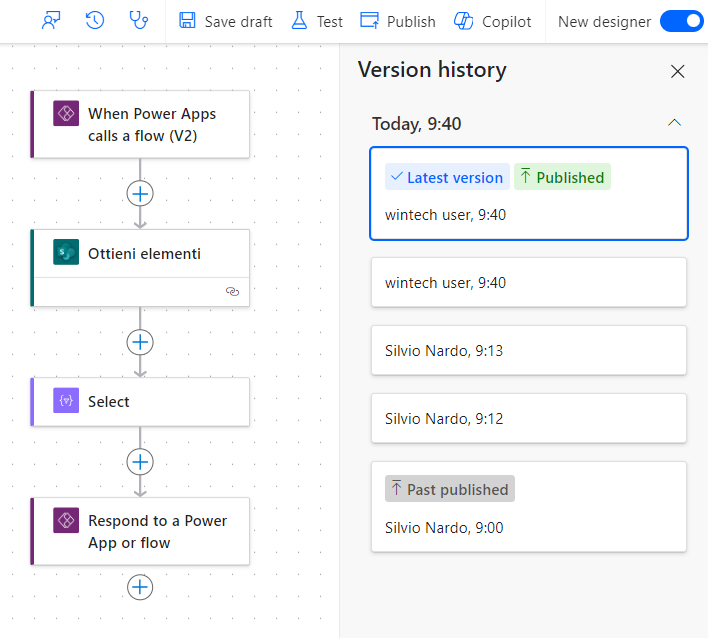
\includegraphics[width=0.8\columnwidth]{versionHistory} 
    \caption{Funzionalità Version history nei flussi Power Automate.}
    \label{fig:versionHistory}
\end{figure}
\newline \noindent Inoltre, essendo i componenti di una Soluzione contenuti in un unico pacchetto esportabile, la gestione dei progetti così organizzati risulta più agevole, soprattutto nelle fasi Build, Code e Deploy. 

\subsubsection*{Job Jenkins}
Riguardo alla scelta del tipo di Job da adottare in Jenkins, è stato individuato il "Multibranch Pipeline Job". Esso permette di collegare un \emph{repository} Git e ha la possibilità di gestire automaticamente una \emph{pipeline} indipendente, contenuta in un apposito \emph{file} chiamato "Jenkinsfile", per ogni \emph{branch}.
Tale Job ha inoltre la possibilità di eseguire automaticamente i Jenkinsfile corrispondenti solo ai \emph{branch} in cui è avvenuta una modifica, rendendo questo strumento ideale per la gestione di progetti Git.\\

\subsection{Soluzioni individuate per le fasi DevOps}
\subsubsection*{Plan}
Come strumenti identificati per la pianificazione delle attività sono stati utilizzati Planner e Taiga.
Essi permettono di categorizzare tutte le attività da assegnare al \emph{team} di sviluppo tramite \emph{tag} e contenitori specifici, i quali definiscono lo stato di avanzamento dei lavori.\\
Nello specifico, Planner viene utilizzato solo dal responsabile di progetto e serve a tenere traccia dei casi d'uso, mentre Taiga si occupa di tracciare i \emph{task} più specifici assegnati ai membri del \emph{team}, il quale si occupa di organizzarli.

\subsubsection*{Code}
Il versionamento di tutte le parti dei progetti realizzati con Power Apps e Power Automate è avvenuto in un singolo \emph{repository} Git in modo da garantire una migliore organizzazione dei dati e facilità di ripristino di specifiche versioni.\\
Per il lavoro collaborativo è stata individuata la \emph{feature} che integra il collegamento ad un \emph{repository} Git con Power Apps e permette di fare \emph{commit} e \emph{push} automaticamente.\\
Il \emph{repository} è diviso nei \emph{branch} "Main", per le versioni funzionanti e stabili del prodotto, "Develop", per il prodotto ancora in fase di sviluppo, e diversi \emph{feature branch} utilizzati dai singoli sviluppatori per apportare modifiche limitate a singole funzioni.\\
Per applicare a tali progetti l'analisi statica del codice, ho individuato come soluzione l'utilizzo degli strumenti nativi offerti da Microsoft:
\begin{itemize}
    \item Verifica flusso: permette l'esecuzione di un controllo sul codice e la visualizzazione di errori sul flusso come i campi obbligatori mancanti, gli \emph{input} non validi o i problemi legati alle licenze. 
    \item Verifica app: permette l'esecuzione di un controllo sul codice e la visualizzazione di errori sull'applicazione come formule Fx non valide, problemi di accessibilità o problemi legati alle origini dati. 
    \item Verifica soluzione: più dettagliata delle precedenti, permette l'esecuzione di un controllo sul codice e la visualizzazione di errori sui componenti della Soluzione.
\end{itemize}
\begin{figure}[htbp] 
    \centering 
    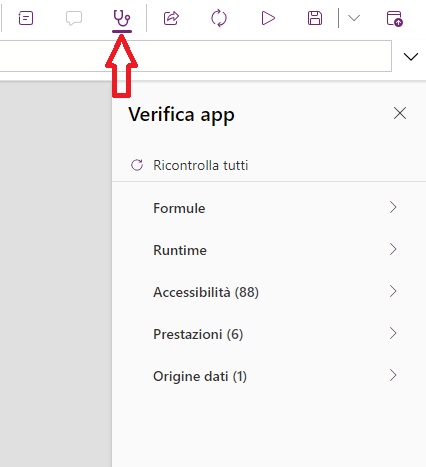
\includegraphics[width=0.6\columnwidth]{verificaApp} 
    \caption{Funzionalità Verifica App nelle applicazioni Power Apps.}
    \label{fig:verificaApp}
\end{figure}

\noindent Gli strumenti di analisi statica esterni non sono stati utilizzati poiché, a seguito di \emph{test} esplorativi e attività di ricerca in merito, è emersa l'eccessiva difficoltà nell'integrazione di qualsiasi strumento non offerto da Microsoft, ai \emph{file} generati dai flussi Power Apps e alle applicazioni Power Automate. 

\subsubsection*{Build}
I \emph{file} generati da Power Automate e Power Apps al fine di rappresentare i flussi e le applicazioni create nelle rispettive interfacce di sviluppo, sono rappresentati da un pacchetto compresso ZIP contenente i \emph{file} generati automaticamente da tali programmi.\\
Essi sono principalmente di tipo JSON, e .msapp e possiedono una struttura di difficile comprensione, pertanto non sono pensati per uno sviluppo manuale diretto.\\
Le Microsoft Solution sono rappresentate dai \emph{file} corrispondenti a quelli dei flussi e delle applicazioni in esse contenuti e nessuno di questi componenti possiede un \emph{file} eseguibile.\\
Come metodo per l'esecuzione della fase Build automatica, ho individuato i comandi forniti dalla Power Platform CLI, automatizzati da un Job Jenkins, al fine di esportare i pacchetti relativi alle Soluzioni desiderate. 

\subsubsection*{Test}
A causa della natura dei pacchetti di dati generati con la fase Build è emerso, similmente all'analisi statica del codice, la necessità di utilizzare principalmente gli strumenti nativi forniti da Microsoft per eseguire \emph{test} dinamici.\\
Per i flussi Power Automate è disponibile la funzione "Test" presente nell'interfaccia grafica di sviluppo.\\
Essa permette l'esecuzione del flusso e la visione dei suoi risultati compresi gli \emph{input} e \emph{output} di ogni azione e il loro tempo di esecuzione. 
Inoltre, in caso di errore, sono fornite le relative informazioni. 
\begin{figure}[htbp] 
    \centering 
    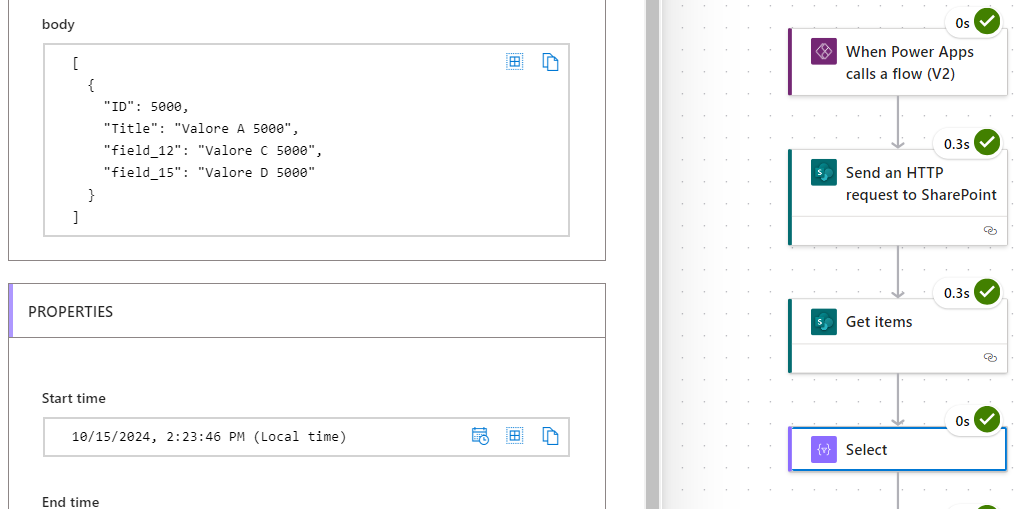
\includegraphics[width=1\columnwidth]{testFlusso} 
    \caption{Funzionalità Test nei flussi Power Automate.}
    \label{fig:testFlusso}
\end{figure}

\newpage \noindent Per eseguire \emph{test} esclusivamente su una specifica parte di un flusso Power Automate, simulando il comportamento delle azioni ad essa connesse, è disponibile la funzione "Static Result".\\
Essa permette un maggiore controllo sull'esecuzione del flusso durante i \emph{test} e l'azzeramento dei tempi di esecuzione di azioni che non rappresentano il suo \emph{focus}.\\
È inoltre stata individuata la possibilità di utilizzare i Trigger e le Azioni Power Automate legate all'utilizzo delle chiamate \gls{http}, al fine di estrapolare i dati di \emph{output} di un flusso ed elaborarli in uno \emph{script} esterno realizzato con l'ambiente Node.js, il quale sfrutta il linguaggio JavaScript. Maggiori informazioni su quanto sviluppato per questa soluzione sono presenti nella parte \hyperref[testProgrammazione]{Test} della sottosezione \hyperref[Sviluppo DevOps]{Sviluppo DevOps}.\\\\
Per quanto concerne i \emph{test} su applicazioni Power Apps, sono presenti diversi strumenti nativi per verificare la loro corretta esecuzione.\\
"Test studio" è uno strumento che permette di eseguire l'applicazione e registrare tutte le azioni intraprese dall'utente (o definite manualmente), al fine di generare uno \emph{script} di \emph{test} che possa ripetere tali azioni e fornire un riscontro.\\
Attualmente l'utilizzo di Test studio non è conveniente a causa del numero considerevole di limitazioni:
il suo funzionamento è limitato solo a componenti "classici", ovvero una lista di componenti presenti su Power Apps prima dell'arrivo dei componenti "moderni".\\
Esclude inoltre l'uso di componenti \emph{custom} e non è compatibile con l'integrazione nativa tra Power Apps e Git.\\\\
Per questi motivi la metodologia identificata per permettere il \emph{testing} ad applicazioni Power Apps è la funzionalità "Visualizza l'anteprima dell'app", con la quale è possibile eseguirla e verificarne il corretto funzionamento.\\
Nel caso in cui si verificassero degli errori durante tale operazione, i loro dettagli possono essere visualizzati. 

\subsubsection*{Release}
La strategia identificata per definire i rilasci è l'assegnazione di specifici \emph{tag} alfanumerici ai \emph{commit} nel \emph{repository} Git.\\
Tale codice è composto dalla lettera "v" seguita da tre cifre separate da un carattere ".", per esempio "v1.0.0".\\
Il criterio di avanzamento delle cifre è: 
\begin{itemize}
    \item Avanzamento della prima cifra: sono avvenute modifiche architetturali che alterano significativamente le funzionalità previste ad alto livello.\\
    Esempio: sostituzione di una tecnologia fondamentale per il funzionamento di un programma o cambiamento radicale dei casi d'uso individuati.  
    \item Avanzamento della seconda cifra: sono avvenute modifiche che alterano le funzionalità previste ad alto livello o ne aggiungono di nuove.\\
    Esempio: modifiche che soddisfano i requisiti di un caso d'uso non ancora risolto, aggiunta di classi in uno \emph{script} che alterano il comportamento precedente del programma, aggiunta di una nuova scheda di un'applicazione.
    \item Avanzamento della terza cifra: sono avvenute modifiche che non alterano significativamente le funzionalità previste ad alto livello.\\
    Esempio: \emph{Bug fix}, sostituzione di un componente di un'applicazione al fine di ottenere il medesimo risultato precedentemente atteso. 
\end{itemize}

\subsubsection*{Deploy}
Power Apps, Power Automate e le Micorsoft Solutions permettono non solo di esportare i pacchetti relativi ai propri progetti, ma anche di importarne di altri.\\
In tale funzione ho individuato il metodo per distribuire i prodotti negli ambienti di produzione. 

\subsubsection*{Operate}
L'operatività delle soluzioni implementate viene monitorata tramite il \emph{feedback} fornito dal cliente.\\
Nel caso in cui si verificasse un problema con tale prodotto, viene fornita immediato supporto al fine di soddisfare nuovamente le attese.\\
Nel caso in cui il problema riscontrato fosse molto problematico, il sistema di versionamento definito permette il ripristino del prodotto ad una precedente versione stabile. 

\subsubsection*{Monitor}
Il monitoraggio dei \emph{report} Jenkins, delle esecuzioni dei flussi Power Automate e delle esecuzioni delle applicazioni Power Apps, sono nativamente forniti dai rispettivi servizi. Tramite le interfacce disponibili è possibile vedere le informazioni sufficienti ad identificare eventuali problemi e "colli di bottiglia".
\begin{figure}[htbp] 
    \centering 
    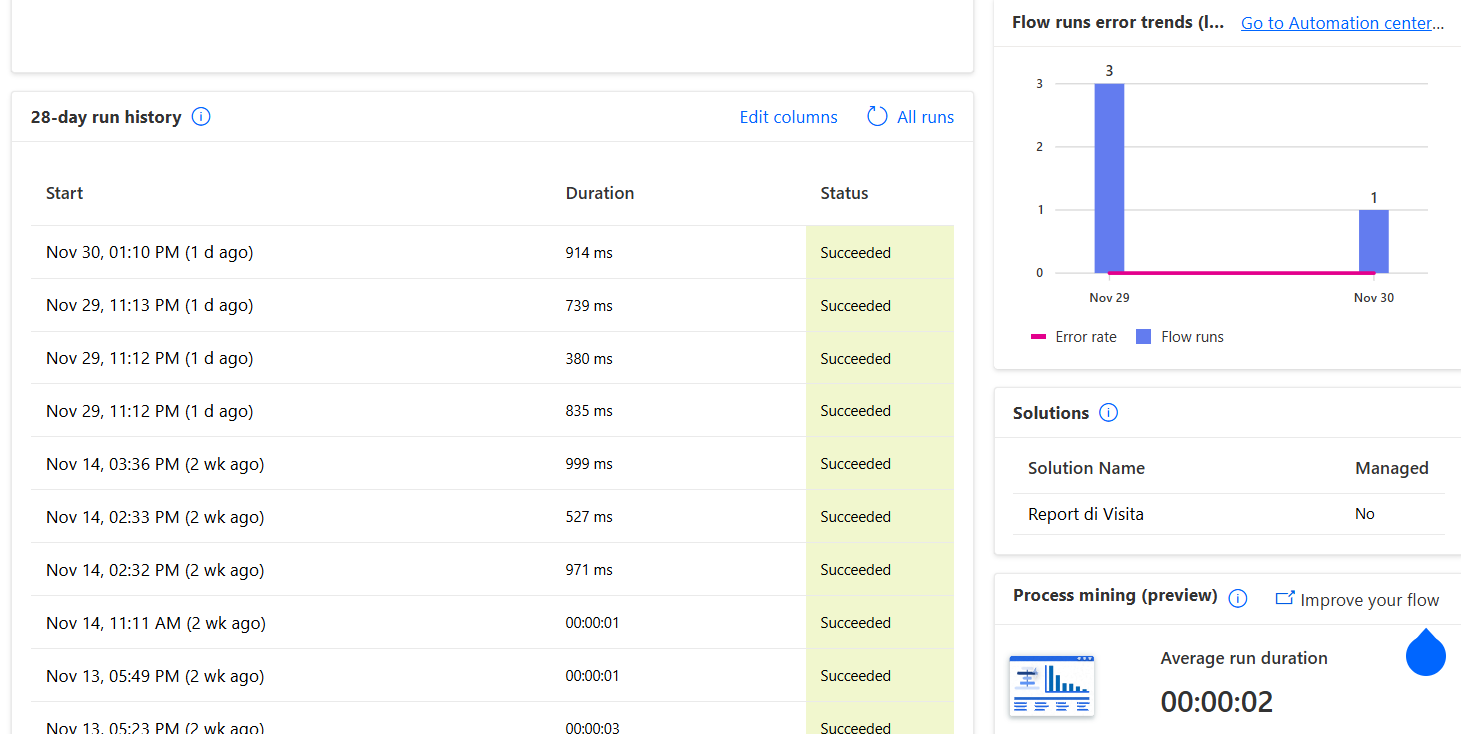
\includegraphics[width=1\columnwidth]{flowMonitor} 
    \caption{Vista parziale dell'interfacccia atta a monitorare un flusso.}
    \label{fig:flowMonitor}
\end{figure}

\newpage \subsection{Progettazione delle applicazioni aziendali}
Le attività di progettazione che ho svolto, relative alle applicazioni aziendali, sono state limitate alla scelta delle strategie da esplorare per risolvere i problemi emersi. Questo perché tali applicazioni erano già presenti da tempo al momento del mio arrivo in azienda.
Eccezione è fatta per l'applicazione "Non conformità" che, a differenza delle altre, era nelle sue prime fasi di sviluppo.\\
Al fine di comprenderne gli obiettivi ho preso parte a dei \emph{meeting} dedicati con il \emph{\emph{tutor}} aziendale e la parte del \emph{team} di sviluppo coinvolta.\\ 
Ho in seguito contribuito a progettare l'aspetto grafico e le soluzioni atte a soddisfarne i requisiti, ma il mio periodo di \emph{stage} è terminato prima che io potessi iniziare il loro sviluppo.  

\section{Codifica e documentazione}
In questa sezione sono presenti tutte le attività da me svolte al fine di sviluppare e implementare le soluzioni individuate in fase di progettazione.
\subsection{PoC iniziali}
Le prime fasi dello \emph{stage} sono state autonome e a supporto della comprensione ed esplorazione delle tecnologie a me richieste. 
Avendo iniziato le mie attività con Power Automate, ho realizzato un primo flusso al fine di testare l'utilizzo di: Trigger, Azioni, collegamento con i servizi Microsoft OneDrive ed Excel, Azioni condizionali, cicli Do until, inizializzazione e modifica di variabili.\\
Tale flusso viene eseguito automaticamente quando viene creato un \emph{file} dentro ad un \emph{path} specifico su OneDrive e di conseguenza invia un'approvazione notificata sia tramite Teams che Outlook.\\
Dopo aver ricevuto la risposta, il flusso agisce di conseguenza spostando il \emph{file} iniziale in un \emph{path} specifico in funzione dell'esito dell'approvazione. Viene in aggiunta eseguito un controllo sui \emph{file} già presenti nel percorso di destinazione e, nel caso fosse già presente un documento omonimo, il documento da spostare viene rinominato.\\
Questo controllo avviene ciclicamente incrementando un valore posto nel nome del \emph{file} fino al verificarsi dell'effettiva possibilità di eseguire lo spostamento.\\
Infine viene eseguito uno \emph{script} Excel il quale scrive in una tabella di \emph{log} le informazioni relative allo spostamento.
\begin{figure}[htbp] 
    \centering 
    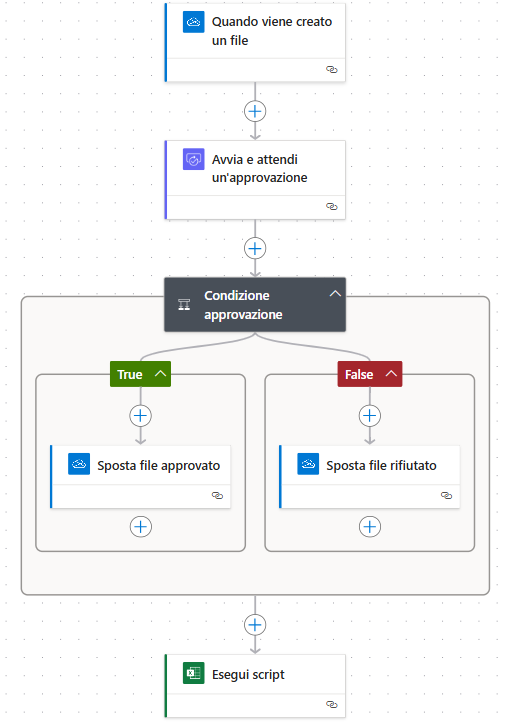
\includegraphics[width=0.5\columnwidth]{flussoApprovazioni} 
    \caption{Flusso per testare condizioni, approvazioni ed esecuzione di \emph{script}.}
    \label{fig:flussoApprovazioni}
\end{figure}
\newline \noindent A fini illustrativi l'immagine mostra una versione semplificata del flusso descritto. Essa esclude il controllo della presenza di un \emph{file} omonimo e quindi non include il ciclo Do until e l'inizializzazione e modifica di variabili.\\
Successivamente, ho prodotto una presentazione PowerPoint al fine di esporre al \emph{\emph{tutor}} aziendale le funzionalità, i lati positivi e i lati negativi delle tecnologie Power Automate e Power Apps, in funzione di quanto appreso durante la prima settimana di \emph{stage}.

\subsection{Sviluppo DevOps}
\label{Sviluppo DevOps}
\subsubsection*{Plan} 
Le attività pratiche legate alla fase di pianificazione sono la configurazione degli ambienti Planner e Taiga e la loro condivisione e utilizzo con i membri del \emph{team} coinvolti.\\
Inoltre, in collaborazione con lo stagista responsabile del progetto \hyperref[stageGiacomo]{Integrazione sistemi di pianificazione di progetto}, abbiamo esplorato la possibilità di integrare i flussi Power Automate al fine di sostituire le logiche, realizzate tramite complessi \emph{scirpt}, responsabili per l'interazione e la sincronizzazione tra le due piattaforme di pianificazione.\\
Per farlo abbiamo inoltre esplorato l'utilizzo dei \emph{webhooks}, ovvero degli strumenti \emph{web} che permettono di configurare l'invio automatico di chiamate \gls{http} di ritorno. Esse vengono eseguite da parte di un'applicazione \emph{web} al fine di permettere dell'utilizzatore di questo strumento di ricevere dati automaticamente al verificarsi di uno specifico evento.\\
A causa delle limitazioni incontrate nell'utilizzo di servizi di \emph{webhooks}, e della fine dello svolgimento dello \emph{stage} della persona con cui collaboravo, tali studi non hanno portato a soluzioni effettivamente utilizzate.

\subsubsection*{Code}
Le attività al fine di predisporre la fase Code, per la sua applicazione a progetti Power Automate e Power Apps, comprendono principalmente la realizzazione e la documentazione del sistema di versionamento individuato in fase di progettazione e la documentazione e l'applicazione degli strumenti per l'analisi statica del codice identificati.\\
Per il versionamento ho adattato, prima in un \emph{branch} di prova e poi nei restanti, il \emph{repository} Git dell'applicazione aziendale Report di visita in modo da rispecchiare le norme definite.
Esse riguardano le regole da seguire per versionare il progetto e la struttura dei percorsi dei \emph{file}, divisi in base alla loro funzione.\\  
Tali norme sono state definite con la collaborazione di parte del \emph{team} di sviluppo e dello stagista universitario responsabile del progetto \hyperref[stageDavide]{Applicativi di DevOps in ambito Sistemi}.\\ 
Per fare in modo di contenere nel \emph{repository} i \emph{file} relativi ai flussi Power Automate e le applicazioni Power Apps, è stata predisposta una cartella apposita al fine di contenere il pacchetto ZIP relativo alla Microsoft Solution del progetto.\\ 
Tale pacchetto nel \emph{repository} assume valore in ottica di \emph{backup} e ripristino, in caso sia necessaria l'esecuzione di una specifica versione del progetto.\\  
Per fare in modo che Power Apps riesca ad utilizzare la funzione integrata che gli permette di interfaccairsi con Git direttamente dalla sua interfaccia grafica, è necessario che nel \emph{repository} sia presente tale applicazione in un formato non compresso. È pertanto stato deciso di mantenere, per quanto ridondante, una copia dell'applicazione al fine di agevolare le fasi di sviluppo.\\ 
Per l'analisi statica del codice ho esplorato altri strumenti esterni come l'applicazione di strumenti di analisi statica consolidati, ad esempio SonarQube, applicati tramite IDE esterni ai dati generati da Power Automate e Power Apps.\\  
Inoltre ho constatato la possibilità di utilizzare gli strumenti diagnostici nativi di tali tecnologie anche tramite i comandi della Power Platform CLI, in modo da automatizzare la raccolta dei risultati.\\ 
Tuttavia, questa funzione risulta superflua, poiché i risultati sono più facilmente accessibili tramite l'interfaccia grafica durante le fasi di sviluppo. Inoltre, perde di utilità se, per verificare lo stato del codice, è necessario eseguire uno \emph{script} e analizzare un complesso \emph{file} JSON.\\ 
I documenti “Norme di progetto” e “Analisi statica” sono stati redatti e sono stati condivisi con il \emph{team} di sviluppo e con il \emph{\emph{tutor}} aziendale.\\  
Infine ho prodotto una presentazione PowerPoint contenente le principali informazioni presenti nei documenti citati e l'ho esposta al \emph{team} di sviluppo. 

\subsubsection*{Build}
Al fine di collegare il Job Jenkins con il \emph{repository}, senza dover utilizzare \emph{token} di accesso GitHub personali, ho utilizzato la funzione che permette di generare “GitHub Apps”. Esse sono applicazioni integrate in GitHub che permettono il collegamento tra i \emph{repository} desiderati con altri specifici strumenti e servizi, definendone con precisione il livello di accesso e autorizzazioni.  
\begin{figure}[htbp] 
    \centering 
    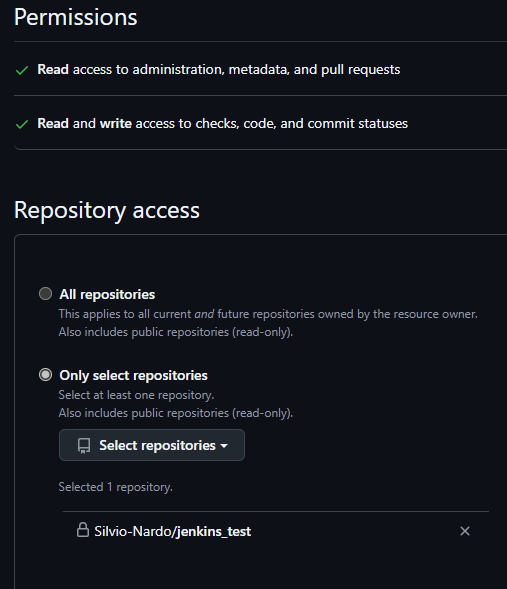
\includegraphics[width=0.4\columnwidth]{githubAppPermessi} 
    \caption{Configurazione dei permessi e selezione dei repository connessi ad una GitHub App.}
    \label{fig:githubAppPermessi}
\end{figure}
\newline Per automatizzare l'esportazione delle Microsoft Solutions e il loro caricamento nel \emph{repository}, ho adottato un Multibranch Pipeline Job Jenkins. Il relativo Jenkinsfile da me prodotto esegue, tramite i propri Stage, le seguenti operazioni:
\begin{itemize}
    \item Seleziona il corretto \emph{branch} del \emph{repository} ed esegue un comando \emph{pull}
    \item Cerca modifiche nella cartella relativa all'applicazione Power Apps
    \item Esegue l'autenticazione Micorsoft tramite gli appositi comandi forniti dalla Power Platform CLI
    \item Esporta la Microsoft Solutions
    \item Controlla l'eventuale presenza di una omonima Solution già presente nel \emph{repository} e, se presente, la elimina 
    \item Carica il pacchetto relativo alla nuova versione della Solution nel \emph{repository}
\end{itemize}
Ho redatto il documento “Guida Jenkins”, il quale comprende tutte le nozioni e le norme relative all'adozione di Jenkins, al fine di applicare la fase Build ai progetti Power Automate e Power Apps e l'ho condiviso con il \emph{team} di sviluppo e con il \emph{\emph{tutor}} aziendale.

\subsubsection*{Test}
\label{testProgrammazione}
L'applicazione di \emph{test} automatici per i flussi Power Automate è avvenuta, oltre all'utilizzo degli strumenti nativi già discussi, tramite lo sviluppo di soluzioni esterne sfruttando le chiamate \gls{http}.
Esse permettono la comunicazione e lo scambio di dati tra flussi Power Automate e altri flussi o applicazioni: esiste infatti la possibilità di richiamare lo specifico Trigger “Alla ricezione di una richiesta HTTP”, il quale genera un personale URL (Uniform Resource Locator), ovvero una sequenza di caratteri che identifica univocamente l'indirizzo di una risorsa su una rete di \emph{computer}.\\
In seguito è possibile utilizzare la corrispondente azione “Response” al fine di rispondere al chiamante con l'\emph{output} della richiesta.\\
\begin{figure}[htbp] 
    \centering 
    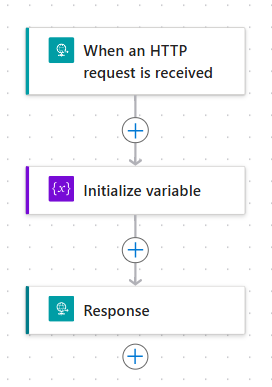
\includegraphics[width=0.3\columnwidth]{flussoHttp} 
    \caption{Flusso di esempio per ricevere e risondere a chiamate HTTP.}
    \label{fig:flussoHttp}
\end{figure}
\newline L'invio delle chiamate e l'analisi dei dati di \emph{output} inviati dal flusso oggetto di \emph{test}, sono avvenute mediante uno \emph{script} Node.js con l'ausilio della libreria “Axios”, la quale offre funzionalità per l'invio e la ricezione asincrona delle chiamate \gls{http}.\\
Per poter inviare una chiamata al flusso desiderato tramite \emph{script}, è necessario ottenere, tramite un'ulteriore chiamata \gls{http}, un \emph{token} Microsoft di autenticazione.
\begin{figure}[htbp] 
    \centering 
    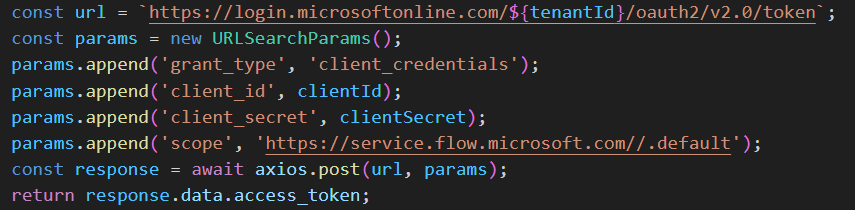
\includegraphics[width=0.8\columnwidth]{richiestaTokenNode} 
    \caption{Parte dello \emph{script} responsabile per l'ottenimento del \emph{token} di autenticazione.}
    \label{fig:richiestaTokenNode}
\end{figure}
\newline In seguito è possibile, aggiungendo l'\emph{output} ottenuto dalla precedente chiamata, inviare la richiesta di esecuzione al flusso da testare.\\
Grazie all'Azione del flusso “Response”, lo \emph{script} può proseguire alla ricezione della risposta contenente l'\emph{output} di Power Automate, in modo da analizzarla e determinarne l'esito.
\begin{figure}[htbp] 
    \centering 
    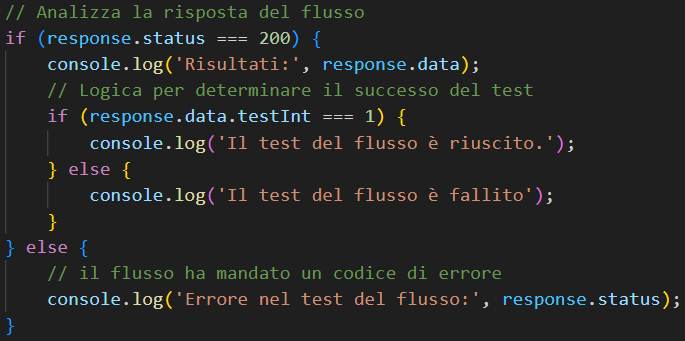
\includegraphics[width=0.6\columnwidth]{analisiEsitoTest} 
    \caption{Parte dello \emph{script} responsabile per l'analisi dell'esito dei \emph{test} su flussi Power Automate.}
    \label{fig:analisiEsitoTest}
\end{figure}
\newline Nell'immagine è mostrata una porzione dello \emph{script} nel quale viene, a fini dimostrativi, controllato se il risultato della chiamata è stata un successo, definito con codice 200, e se l'\emph{output} del flusso è uguale ad un intero di valore 1. In funzione dell'esito del controllo e dello stato di successo della chiamata, viene mostrato a schermo un relativo messaggio.\\
Ai fini di rendere automatico questo processo, l'esecuzione dello \emph{script} illustrato è stato incluso nel Jenkinsfile relativo al Job Jenkins dell'applicazione aziendale Report di visita.
Tale pratica garantisce la qualità e la funzionalità attesa dai flussi testati, però è da considerare che la natura dei prodotti realizzati con Power Automate richiede che essi vengano modificati, al fine di essere predisposti alla ricezione e alla risposta delle chiamate \gls{http} di \emph{test}. Inoltre è da tenere in considerazione che tali funzioni necessitano della licenza \emph{premium}.\\\\
Per le applicazioni Power Apps ho esplorato la possibilità di estrarre, tramite la funzione “Scarica suite”, un \emph{file} contenente le azioni registrate dallo strumento Test Studio ma, in funzione delle conclusioni esplicitate precedentemente riguardo tale strumento, la strategia non è stata integrata nel sistema di \emph{testing}.\\\\
Ho prodotto il documento “Test dinamici”, contenente tutte le informazioni relative ai metodi individuati per effettuare tali \emph{test} su Power Automate e su Power Apps, sia con strumenti nativi che esterni. Ho aggiornato il documento “Guida Jenkins” al fine di contenerne anche le nozioni riguardanti quanto descritto.\\
Tali documenti sono stati condivisi con il \emph{team} di sviluppo e con il \emph{\emph{tutor}} aziendale.\\
Inoltre ho prodotto, ed esposto al \emph{team} di sviluppo, una presentazione PowerPoint contenente le principali informazioni apprese e le soluzioni individuate e sviluppate relativamente alle fasi Build e Test. 

\subsubsection*{Deploy}
Al fine di comprendere e testare l'applicazione della fase Deploy ho esplorato, insieme a parte del \emph{team} di sviluppo, le funzionalità legate all'importazione delle Microsoft Solutions, gestite e non gestite, all'interno di diversi ambienti di produzione.\\ 
Al fine di agevolare il collegamento agli \emph{account} e ai servizi Microsoft corrispondenti al nuovo ambiente, sono state utilizzate, ed inserite all'interno della relativa Solution, i “riferimenti alle connessioni”. Essi sono entità che rappresentano il collegamento tra un'applicazione, un servizio o un flusso e una risorsa esterna, e offrono la possibilità di essere cambiati in maniera dinamica durante la fase di importazione in un ambiente.\\\\
L'applicazione delle fasi di \gls{DevOps} Release, Operate e Monitor, a seguito delle attività di analisi e progettazione, non hanno avuto necessità di attività di sviluppo aggiuntive. 

\subsection{Attività sulle applicazioni aziendali}
\label{sviluppoApplicazioni}
\subsubsection*{Report di visita}
Le attività di sviluppo dell'applicazione aziendale Report di visita hanno affiancato le attività di ricerca del mio \emph{stage} per la maggior parte della sua durata.\\
Esse, oltre all'integrazione delle pratiche \gls{DevOps} descritte precedentemente, si sono focalizzate sulle strategie di \emph{retrieve} dei dati tramite appositi flussi Power Automate collegati all'applicazione.\\
Lo strumento di archiviazione utilizzato principalmente è stato SharePoint, ma è stata testata anche la possibilità \emph{premium} di leggere dati da SQL Server.\\
Le principali difficoltà affrontate sono relative ai limiti sul numero di \emph{record} ottenibili per ogni richiesta a SharePoint:
\begin{itemize}
    \item Essendo per Power Apps una funzione non delegabile, ovvero che non può delegare l'elaborazione dei dati al \emph{server}, è presente il limite di 500 \emph{record} ottenibili di \emph{default} estendibile fino a 2000 modificando le impostazioni. Inoltre eventuali filtri sulla ricerca vengono applicati solo dopo aver ricevuto quel numero di dati, pertanto, il risultato ottenuto è un insieme limitato del risultato atteso.
    \item Eseguendo l'analoga funzione da un flusso Power Automate, si incorre in un ulteriore limite imposto da Sharepoint uguale a 5000 risultati ottenibili per chiamata.\\
    In merito sono state esplorate soluzioni legate al precaricamento di tutti i dati, mediante chiamate multiple, al fine di applicare successivamente il filtraggio dei dati richiesti, e all'utilizzo di chiamate \gls{http} a servizi SharePoint. Queste soluzioni sono state successivamente scartate a causa degli eccessivi tempi di esecuzione e ad altre limitazioni incontrate, come l'impossibilità per SarePoint di eseguire il comando di ricerca per sottostringa.
    \item Dopo aver ottenuto i dati desiderati, sfruttando particolari funzionalità di indicizzazione delle liste SharePoint, sono state incontrate difficoltà legate all'aggiornamento grafico di alcuni componenti fondamentali dell'applicazione utilizzati per mostrare dinamicamente i contenuti ricavati.\\
    Tale problema è stato risolto tramite lo sviluppo di un nuovo componente \emph{custom}.  
\end{itemize}
Al fine di fare \emph{test} su liste SharePoint, popolate dinamicamente da un numero elevato di elementi, ho generato tabelle Excel in maniera automatica scrivendo appositamente degli “Office Scripts”.\\
Le mie attività di sviluppo legate alle applicazioni Registro accessi e "Non conformità" sono legate ad aspetti grafici e all'individuazione di possibili risoluzioni di problemi legati alle singole funzioni Fx. 

\subsection{Attività con Angular}
Al fine di comprendere il funzionamento e lo sviluppo di progetti basati su Angular, ho realizzato una basilare applicazione \emph{web} che mostrava nell'interfaccia grafica immagini e testo.\\
Essa è stata il punto di partenza per lo sviluppo di una \emph{suite} di \emph{test} eseguiti con l'apposito strumento “Karma”. Tale esecuzione è poi stata automatizzata in un Job Jenkins di tipo \emph{pipeline}, il quale: 
\begin{itemize}
    \item Seleziona e utilizza la versione di Node.js predeterminata
    \item Preleva il progetto dal \emph{repository} Git
    \item Esegue i \emph{test} di unità definiti
    \item Compila i \emph{file} e genera il relativo pacchetto composto da elementi HTML e JavaScript
    \item Mostra a schermo il risultato dei \emph{test} in un apposito grafico
    \item Salva gli artefatti creati in Jenkins, vincolando la presenza dei salvataggi ai soli tre più recenti
    \item Pulisce il \emph{workspace} relativo al Job e alle compilazioni avvenute  
\end{itemize}
\begin{figure}[htbp] 
    \centering 
    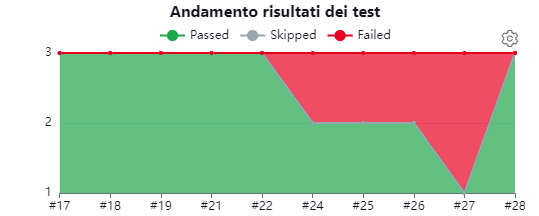
\includegraphics[width=0.7\columnwidth]{graficoTest} 
    \caption{Grafico dell'esito dei \emph{test} generato da Jenkins.}
    \label{fig:graficoTest}
\end{figure}
Inoltre ho applicato quanto appreso per produrre un ulteriore \emph{pipeline} Job al fine di replicare le fasi di \gls{DevOps} anche su progetti aziendali realizzati con Angular.\\
Infine ho generato il documento “Angular in Jenkins” contenente quanto affrontato in merito e l'ho esposto al \emph{team} di sviluppo e al \emph{\emph{tutor}} aziendale. 

\section{Risultati raggiunti}
\subsection{Risultati qualitativi}
Lo studio delle tecnologie Power Automate e Power Apps ha fatto emergere la loro natura: essi sono \emph{software} utili nei casi in cui si debba realizzare un'applicazione semplice rapidamente, ma è da considerare che sono strumenti ancora relativamente nuovi, quindi privi di una documentazione esaustiva e aventi \emph{features} soggette a frequenti e importanti modifiche.\\
Offrono la possibilità di connettersi agevolmente con i servizi Microsoft ma presentano allo stesso tempo un alto numero di limitazioni, le quali non offrono la libertà di sviluppo ottenibile con i consolidati strumenti e linguaggi di programmazione.\\ 
Lo studio da me svolto durante lo \emph{stage} ha fatto emergere l'effettiva possibilità di applicare le metodologie \gls{DevOps} a progetti realizzati con Power Auotmate e Power Apps.\\\\
Tramite periodi di sviluppo collaborativo, ho dimostrato la possibilità di applicare strategie di collaborazione e condivisione delle risorse tra membri del \emph{team} di sviluppo.\\ 
Ho definito le norme di versionamento che il \emph{team} deve seguire per organizzare efficacemente tutte le parti che compongono un progetto Power Automate/Power Apps, testando la possibilità di effettuare il ripristino di specifiche versioni rilasciate.\\ 
Ho applicato metodologie di analisi statica del codice e \emph{testing} dinamico, sia mediante strumenti nativi che esterni, al fine di verificare il corretto funzionamento e garantire la qualità dei prodotti realizzati.\\ 
Ho dimostrato la possibilità di gestire il ciclo di vita del \emph{software} prodotto, relativamente alle tecnologie in oggetto, comprese le fasi di distribuzione dei prodotti e il loro monitoraggio.\\ 
Ogni nozione da me acquisita, ogni norma stipulata e ogni soluzione implementata è stata documentata ed è stata resa disponibile al personale attraverso gli strumenti di condivisione aziendale. 

\subsection{Risultati qualitativi}
\begingroup
\renewcommand\arraystretch{1.3}
\begin{longtable}{|p{11cm}|}
    \caption{Documenti che ho prodotto durante lo \emph{stage}.}
    \label{tab:risultatiQualitativi}\\
    \hline \multicolumn{1}{|c|}{\textbf{Documenti prodotti}}\\ \hline \endfirsthead
    \hline \multicolumn{1}{|c|}{\textbf{Documenti prodotti}}\\ \hline \endhead
    \hline \endhead
    \hline \endfoot
    \hline \endlastfoot
    \hline “Analisi statica del codice”\\
    \hline “Norme di versionamento”\\
    \hline “Test dinamici”\\
    \hline “Guida Jenkins”\\
    \hline “Angular in Jenkins”\\
    \hline Presentazione sulle funzionalità, i lati positivi e i lati negativi di Power Automate e Power Apps\\
    \hline Presentazione relativa alle limitazioni di tali tecnologie e le rispettive soluzioni individuate\\
    \hline Presentazione relativa al versionamento e all'analisi statica del codice\\
    \hline Presentazione relativa ai processi Build e ai \emph{test} dinamici\\
    \hline Presentazione finale realizzata in collaborazione con gli altri stagisti universitari riguardo a quanto fatto durante i nostri \emph{stage}\\
\end{longtable}
\endgroup
 
\subsection{Risultati quantitativi}
\begingroup
\renewcommand\arraystretch{1.3}
\begin{longtable}{|p{11cm}|}
    \caption{Software che ho prodotto durante lo \emph{stage}.}
    \label{tab:risultatiQuantitativi}\\
    \hline \multicolumn{1}{|c|}{\textbf{Software prodotti}}\\ \hline \endfirsthead
    \hline \multicolumn{1}{|c|}{\textbf{Software prodotti}}\\ \hline \endhead
    \hline \endfoot
    \hline \endlastfoot
    \hline PoC sui flussi approvativi\\
    \hline PoC sull'integrazione di chiamate \gls{http} con i flussi\\
    \hline Jenkinsfile per progetti Power Automate/Power Apps\\
    \hline \emph{Script} Excel per la creazione automatica di tabelle\\
    \hline \emph{Script} Node.js per il \emph{test} di flussi tramite chiamate \gls{http}\\
    \hline Sviluppo di funzioni Fx sul prodotto aziendale Report di visita\\
    \hline Flussi per il \emph{retreive} dei dati da liste SharePoint\\
    \hline Progetto di esempio Angular\\
    \hline Jenkinsfile relativo al progetto di esempio Angular\\
\end{longtable}
\endgroup


    \chapter{Valutazione retrospettiva}
\label{cap:valutazioneRetrospettiva}
\section{Raggiungimento obiettivi}
In riferimento alla tabella degli obiettivi LINKALLATABELLA, in seguito vengono riportate le azioni da me intraprese al fine di raggiungere il loro soddisfacimento e i corrispondenti esiti.

\begingroup
\renewcommand\arraystretch{1.3}
\begin{longtable}{|c|p{8cm}|c|}
    \caption{Soddisfacimento degli obiettivi obbligatori.}
    \label{tab:soddObbObbligatori}\\
    \hline \textbf{Requisito} & \textbf{Azioni risolutive} & \textbf{Esito}\\ \endfirsthead
    \hline \textbf{Requisito} & \textbf{Azioni risolutive} & \textbf{Esito}\\ \endhead
    \hline \endfoot
    \hline \endlastfoot
    \hline O1.1  & A seguito dell'analisi svolta sui flussi Power Automate, ho compreso le informazioni relative alle sue funzionalità, caratteristiche, punti positivi e punti negativi. Ho redatto il documento “Presentazione Power Automate e Power Apps” al fine di esporre il risultato di tali ricerche. & Soddisfatto\\
    \hline O1.2  & Ho prodotto molteplici flussi Power Automate: flussi per il \emph{retrive} dei dati da SharePoint, flussi di approvazione e per l'integrazione con chiamate \gls{http}. & Soddisfatto\\
    \hline O1.3  & Il documento “Presentazione Power Automate e Power Apps” è stato esposto e discusso con il \emph{tutor} aziendale e con il \emph{team} di sviluppo. & Soddisfatto\\
    \hline \textbf{O1}    & Ho studiato, analizzato ed esplorato la tecnologia Power Automate, redigendo i relativi documenti, i quali ho poi condiviso con il \emph{team} aziendale. & Soddisfatto\\
    \hline O2.1  & Ho affiancato il membro del \emph{team} di sviluppo responsabile della realizzazione dei prodotti Power Apps aziendali. Egli mi ha spiegato dettagliatamente il funzionamento del programma e delle applicazioni create. & Soddisfatto\\
    \hline O2.2  & Ho individuato, come sistema per lo sviluppo collaborativo di applicazioni Power Apps, la condivisione del materiale su Git mediante l'apposito comando integrato. Ho redatto il documento “Norme di versionamento” al fine di normare e standardizzare il suo utilizzo e le strategie di collaborazione. & Soddisfatto\\
    \hline O2.3  & Ho sviluppato, collaborativamente e autonomamente, flussi Power Automate e formule Power Fx, ottenendo avanzamenti nello stato dei lavori di applicazioni aziendali realizzate con Power Apps. & Soddisfatto\\
    \hline \textbf{O2}  & Ho studiato Power Apps mediante ricerca individuale e formazione collaborativa. Ho ottenuto avanzamenti nello stato dei lavori su applicazioni aziendali realizzate con tale tecnologia. & Soddisfatto\\
    \hline \textbf{O3}  & Ho individuato, analizzato, testato ed applicato un sistema per il versionamento di progetti realizzati con Power Automate e Power Apps basato su \emph{repository} Git. Le norme relative al suo utilizzo sono state approvate dal \emph{team} di sviluppo e sono state da me descritte approfonditamente nel documento “Norme di versionamento”. & Soddisfatto\\
    \hline \textbf{O4}  & Ho studiato la metodologia \gls{DevOps} e tutte le sue fasi. Ho studiato le possibilità di applicarle alle tecnologie Power Automate e Power Apps, individuando soluzioni specifiche che ho poi sviluppato e integrato ai relativi progetti aziendali. Al fine di condividere con il \emph{team} tali informazioni, ho redatto i documenti “Norme di versionamento”, “Analisi statica del codice” e “Test dinamici”. Inoltre, al fine di descrivere la tecnologia utilizzata per gestire la maggior parte di queste fasi, ho redatto il documento “Guida Jenkins”. & Soddisfatto\\
\end{longtable}

\begin{longtable}{|c|p{8cm}|c|}
    \caption{Soddisfacimento degli obiettivi desiderabili.}
    \label{tab:soddObbDesiderabili}\\
    \hline \textbf{Requisito} & \textbf{Azioni risolutive} & \textbf{Esito}\\ \endfirsthead
    \hline \textbf{Requisito} & \textbf{Azioni risolutive} & \textbf{Esito}\\ \endhead
    \hline \endfoot
    \hline \endlastfoot
    \hline \textbf{D1}  & Ho collaborato con gli altri due stagisti universitari al fine di condividere reciprocamente, mediante appositi \emph{meeting} e condivisione dei documenti prodotti, le attività svolte e le nozioni apprese durante i nostri \emph{stage}. Ho con loro collaborato al fine di individuare una soluzione che sincronizzasse gli strumenti Planner e Taiga mediante flussi Power Automate. Inoltre abbiamo discusso e definito parte delle strategie da adottare relativamente al sistema di versionamento per progetti Power Automate e Power Apps. & Soddisfatto\\
    \hline D2.1  & Ho realizzato un flusso Power Automate al fine di dimostrare la fattibilità tecnologica di flussi in grado di inviare richieste di approvazione e reagire contestualmente alla risposta ricevuta. & Soddisfatto\\
    \hline D2.2  & Ho realizzato un flusso Power Automate per dimostrare la fattibilità tecnologica di flussi in grado di ricevere e inviare chiamate \gls{http}, al fine di scambiare dati con \emph{script} e servizi esterni. & Soddisfatto\\
    \hline D2.3  & Ho realizzato un Multibranch \emph{pipeline} Job Jenkins, e relativo Jenkinsfile, al fine di dimostrare l'applicabilità della fase \emph{Build} di \gls{DevOps} a progetti realizzati con Power Automate e Power Apps. Esso include uno \emph{Stage} responsabile per l'esportazione dei prodotti \emph{software}, sotto forma di pacchetti, e il loro caricamento nel \emph{repository} Git. & Soddisfatto\\
    \hline D2.4  & Ho realizzato un Multibranch \emph{pipeline} Job Jenkins, e relativo Jenkinsfile, al fine di dimostrare l'applicabilità della fase \emph{Test} di \gls{DevOps} a progetti realizzati con Power Automate e Power Apps. Esso include uno \emph{Stage} responsabile per l'esecuzione di uno \emph{script} il quale, tramite chiamate \gls{http}, esegue un flusso Power Automate ottenendone l'\emph{output}. Quest'ultimo viene poi automaticamente analizzato al fine di testarne la correttezza. & Soddisfatto\\
    \hline \textbf{D2}  & Ho testato le soluzioni individuate durante l'analisi e la progettazione mediante dimostrazioni e PoC. Ho poi condiviso con il \emph{team} i documenti relativi ai risultati ottenuti, i quali comprendono i PoC sull'utilizzo di Jenkins e alle \emph{features} disponibili con l'utilizzo di flussi Power Automate. & Soddisfatto\\
    \hline \textbf{D3}  & Ho collaborato con lo stagista universitario incaricato di analizzare l'applicabilità delle pratiche \gls{DevOps} in ambito \gls{Sistemi}, al fine di comprenderne le soluzioni individuate, i limiti tecnologici e i benefici guadagnati. Questo è avvenuto tramite appositi \emph{meeting} e condivisione dei documenti redatti. & Soddisfatto\\
\end{longtable}

\begin{longtable}{|c|p{8cm}|c|}
    \caption{Soddisfacimento degli obiettivi facoltativi.}
    \label{tab:soddObbFacoltativi}\\
    \hline \textbf{Obiettivo} & \textbf{Azioni risolutive} & \textbf{Esito}\\  \endfirsthead
    \hline \textbf{Obiettivo} & \textbf{Azioni risolutive} & \textbf{Esito}\\  \endhead
    \hline \endfoot
    \hline \endlastfoot
    \hline \textbf{F1}  & Ho studiato ed esplorato lo strumento Angular, e con esso ho realizzato un'applicazione \emph{web} contenente testo e immagini. & Soddisfatto\\
    \hline \textbf{F2}  & Ho applicato le principali fasi di \gls{DevOps} al progetto Angular da me realizzato, mediante l'utilizzo di un \emph{pipeline} Job Jenkins. & Soddisfatto\\
    \hline \textbf{F3}  & Ho realizzato, in collaborazione con gli altri stagisti universitari, una presentazione finale contenente tutti i risultati raggiunti durante lo \emph{stage}. Essa è stata poi esposta al presidente di Wintech e ai responsabili. & Soddisfatto\\
\end{longtable}
\endgroup

\section{Maturazione professionale}
Nel periodo di \emph{stage} ho affrontato diverse sfide a me nuove in ambito lavorativo, le quali hanno permesso una mia crescita a livello professionale e l'acquisizione di nuove competenze.
Tra queste è compresa la capacità di compiere analisi approfondite riguardo a tecnologie non precedentemente affrontate, l'individuazione degli strumenti da adottare all'interno di un progetto e l'autoapprendimento relativo al loro utilizzo.\\
Ho maturato la capacità di produrre documentazione professionale, conforme agli \emph{standard} aziendali, atta a condividere i risultati delle mie ricerche e a normare processi lavorativi.\\ 
Ho sviluppato competenze relative alla collaborazione con i responsabili e con i \emph{team} aziendali organizzando \emph{meeting}, utilizzando correttamente le tecnologie designate e tramite le fasi di progettazione e sviluppo cooperativo.\\
Ho acquisito ulteriore esperienza relativamente all'autogestione delle attività, al fine di raggiungere gli obiettivi previsti nei tempi e con gli strumenti prestabiliti, mantenendo il rispetto per la qualità attesa e i processi aziendali definiti.\\
Infine, ho sviluppato le mie capacità espositive e comunicative eseguendo presentazioni strutturate e professionali, al fine di condividere le informazioni relative al lavoro da me svolto.\\\\
Ritengo che questa sia stata un'esperienza assolutamente positiva, durante la quale ho collaborato con persone disponibili e propositive, acquisendo nuove competenze e guadagnando esperienza. 

\section{Divario formativo}
Durante lo svolgimento dello \emph{stage}, ho potuto constatare come la formazione universitaria da me intrapresa mi abbia preparato ad affrontare diversi argomenti incontrati nell'ambiente lavorativo.\\
Tra questi sono comprese le filosofie Agile e Scrum, la gestione del ciclo di vita del \emph{software}, le metodologie di automazione \gls{Continuous Integration} e \gls{Continuous Deployment}, e lo scopo delle fasi di \gls{DevOps}.\\
Inoltre ritengo che il progetto universitario compreso nell'insegnamento "Ingegneria del Software", sia stato fondamentale per comprendere come affrontare un progetto, enfatizzando l'importanza dell'analisi, progettazione e redazione dei relativi documenti normativi.\\
Per quanto concerne l'ambito tecnologico, avevo precedentemente affrontato i temi riguardanti le tecnologie Git e Jenkins, e avevo necessariamente già utilizzato IDE e la maggior parte dei linguaggi di programmazione utilizzati durante lo \emph{stage}.\\ 
In ambito informatico esistono una moltitudine di differenti tecnologie, le quali vengono frequentemente aggiornate e modificate. 
Per questo motivo, il corso universitario mi ha formato al fine di apprendere efficacemente nuovi strumenti e tecnologie in autonomia. 


    %\chapter{Introduzione}
\label{cap:introduzione}

Introduzione al contesto applicativo.\\

\noindent Esempio di utilizzo di un termine nel glossario \\
\gls{api}. \\

\noindent Esempio di citazione in linea \\
\cite{site:agile-manifesto}. \\

\noindent Esempio di citazione nel pie' di pagina \\
citazione\footcite{womak:lean-thinking} \\

\section{L'azienda}

Descrizione dell'azienda.

\section{L'idea}

Introduzione all'idea dello stage.

\section{Organizzazione del testo}

\begin{description}
    \item[{\hyperref[cap:processi-metodologie]{Il secondo capitolo}}] descrive ...
    
    \item[{\hyperref[cap:descrizione-stage]{Il terzo capitolo}}] approfondisce ...
    
    \item[{\hyperref[cap:analisi-requisiti]{Il quarto capitolo}}] approfondisce ...
    
    \item[{\hyperref[cap:progettazione-codifica]{Il quinto capitolo}}] approfondisce ...
    
    \item[{\hyperref[cap:verifica-validazione]{Il sesto capitolo}}] approfondisce ...
    
    \item[{\hyperref[cap:conclusioni]{Nel settimo capitolo}}] descrive ...
\end{description}

Riguardo la stesura del testo, relativamente al documento sono state adottate le seguenti convenzioni tipografiche:
\begin{itemize}
	\item gli acronimi, le abbreviazioni e i termini ambigui o di uso non comune menzionati vengono definiti nel glossario, situato alla fine del presente documento;
	\item per la prima occorrenza dei termini riportati nel glossario viene utilizzata la seguente nomenclatura: \emph{parola}\glsfirstoccur;
	\item i termini in lingua straniera o facenti parti del gergo tecnico sono evidenziati con il carattere \emph{corsivo}.
\end{itemize}

    %\chapter{Processi e metodologie}
\label{cap:processi-metodologie}

\intro{Brevissima introduzione al capitolo}\\

\section{Processo sviluppo prodotto}

    %\chapter{Descrizione dello stage}
\label{cap:descrizione-stage}

\intro{Breve introduzione al capitolo}\\

\section{Introduzione al progetto}

\section{Analisi preventiva dei rischi}

Durante la fase di analisi iniziale sono stati individuati alcuni possibili rischi a cui si potrà andare incontro.
Si è quindi proceduto a elaborare delle possibili soluzioni per far fronte a tali rischi.\\

\begin{risk}{Performance del simulatore hardware}
    \riskdescription{le performance del simulatore hardware e la comunicazione con questo potrebbero risultare lenti o non abbastanza buoni da causare il fallimento dei test}
    \risksolution{coinvolgimento del responsabile a capo del progetto relativo il simulatore hardware}
    \label{risk:hardware-simulator} 
\end{risk}

\section{Requisiti e obiettivi}


\section{Pianificazione}

    %\chapter{Analisi dei requisiti}
\label{cap:analisi-requisiti}

\intro{Breve introduzione al capitolo}\\

\section{Casi d'uso}

Per lo studio dei casi di utilizzo del prodotto sono stati creati dei diagrammi.
I diagrammi dei casi d'uso (in inglese \emph{Use Case Diagram}) sono diagrammi di tipo \gls{uml} dedicati alla descrizione delle funzioni o servizi offerti da un sistema, così come sono percepiti e utilizzati dagli attori che interagiscono col sistema stesso.
Essendo il progetto finalizzato alla creazione di un tool per l'automazione di un processo, le interazioni da parte dell'utilizzatore devono essere ovviamente ridotte allo stretto necessario. Per questo motivo i diagrammi d'uso risultano semplici e in numero ridotto.

\begin{figure}[!h] 
    \centering 
    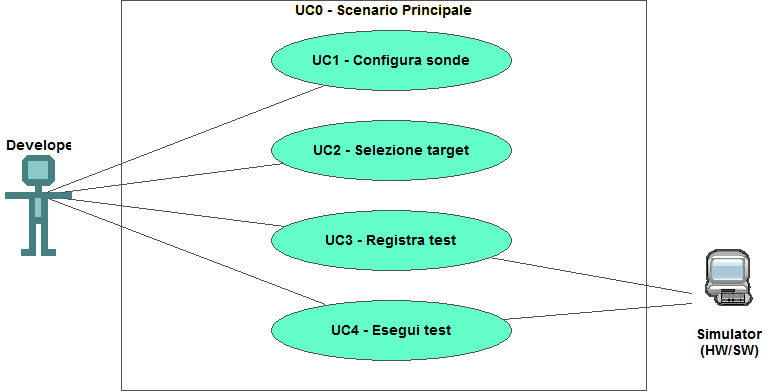
\includegraphics[width=0.9\columnwidth]{usecase/scenario-principale} 
    \caption{Use Case - UC0: Scenario principale}
\end{figure}

\begin{usecase}{0}{Scenario principale}
\usecaseactors{Sviluppatore applicativi}
\usecasepre{Lo sviluppatore è entrato nel plug-in di simulazione all'interno dell'IDE}
\usecasedesc{La finestra di simulazione mette a disposizione i comandi per configurare, registrare o eseguire un test}
\usecasepost{Il sistema è pronto per permettere una nuova interazione}
\label{uc:scenario-principale}
\end{usecase}

\section{Tracciamento dei requisiti}

Da un'attenta analisi dei requisiti e degli use case effettuata sul progetto è stata stilata la tabella che traccia i requisiti in rapporto agli use case.\\
Sono stati individuati diversi tipi di requisiti e si è quindi fatto utilizzo di un codice identificativo per distinguerli.\\
Il codice dei requisiti è così strutturato R(F/Q/V)(N/D/O) dove:
\begin{enumerate}
	\item[R =] requisito
    \item[F =] funzionale
    \item[Q =] qualitativo
    \item[V =] di vincolo
    \item[N =] obbligatorio (necessario)
    \item[D =] desiderabile
    \item[Z =] opzionale
\end{enumerate}
Nelle tabelle \ref{tab:requisiti-funzionali}, \ref{tab:requisiti-qualitativi} e \ref{tab:requisiti-vincolo} sono riassunti i requisiti e il loro tracciamento con gli use case delineati in fase di analisi.

\newpage

\begin{table}%
\caption{Tabella del tracciamento dei requisti funzionali}
\label{tab:requisiti-funzionali}
\begin{tabularx}{\textwidth}{lXl}
\hline\hline
\textbf{Requisito} & \textbf{Descrizione} & \textbf{Use Case}\\
\hline
RFN-1     & L'interfaccia permette di configurare il tipo di sonde del test & UC1 \\
\hline
\end{tabularx}
\end{table}%

\begin{table}%
\caption{Tabella del tracciamento dei requisiti qualitativi}
\label{tab:requisiti-qualitativi}
\begin{tabularx}{\textwidth}{lXl}
\hline\hline
\textbf{Requisito} & \textbf{Descrizione} & \textbf{Use Case}\\
\hline
RQD-1    & Le prestazioni del simulatore hardware deve garantire la giusta esecuzione dei test e non la generazione di falsi negativi & - \\
\hline
\end{tabularx}
\end{table}%

\begin{table}%
\caption{Tabella del tracciamento dei requisiti di vincolo}
\label{tab:requisiti-vincolo}
\begin{tabularx}{\textwidth}{lXl}
\hline\hline
\textbf{Requisito} & \textbf{Descrizione} & \textbf{Use Case}\\
\hline
RVO-1    & La libreria per l'esecuzione dei test automatici deve essere riutilizzabile & - \\
\hline
\end{tabularx}
\end{table}%

    %\chapter{Progettazione e codifica}
\label{cap:progettazione-codifica}

\intro{Breve introduzione al capitolo}\\

\section{Tecnologie e strumenti}
\label{sec:tecnologie-strumenti}

Di seguito viene data una panoramica delle tecnologie e strumenti utilizzati.

\subsection*{Tecnologia 1}
Descrizione Tecnologia 1.

\subsection*{Tecnologia 2}
Descrizione Tecnologia 2

\section{Ciclo di vita del software}
\label{sec:ciclo-vita-software}

\section{Progettazione}
\label{sec:progettazione}

\subsubsection{Namespace 1} %**************************
Descrizione namespace 1.

\begin{namespacedesc}
    \classdesc{Classe 1}{Descrizione classe 1}
    \classdesc{Classe 2}{Descrizione classe 2}
\end{namespacedesc}


\section{Design Pattern utilizzati}

\section{Codifica}

    %\chapter{Verifica e validazione}
\label{cap:verifica-validazione}

    %\chapter{Conclusioni}
\label{cap:conclusioni}

\section{Consuntivo finale}

\section{Raggiungimento degli obiettivi}

\section{Conoscenze acquisite}

\section{Valutazione personale}


    \appendix
    %\chapter{Appendice A}

\epigraph{Citazione}{Autore della citazione}


    \backmatter
    %\printglossary[type=\acronymtype, title=Acronimi e abbreviazioni, toctitle=Acronimi e abbreviazioni]
    \printglossary[type=main, title=Glossario, toctitle=Glossario]

    \cleardoublepage
\chapter{Bibliografia}

\nocite{*}

% Print book bibliography
\printbibliography[heading=subbibliography,title={Riferimenti bibliografici},type=book]

% Print site bibliography
\printbibliography[heading=subbibliography,title={Siti web consultati},type=online]

\end{document}
